% !TEX program = pdflatex
\documentclass[10pt,letterpaper]{article}
\usepackage[T1]{fontenc}
\usepackage{lmodern,amsmath,amssymb,booktabs,graphicx,microtype,array,tabularx}
\usepackage[margin=.75in,headheight=14pt]{geometry}
\usepackage{subcaption,float,placeins,xcolor,fancyhdr,tikz}
\usetikzlibrary{arrows.meta}
\usepackage[colorlinks=true,linkcolor=blue!40!black,urlcolor=blue!40!black]{hyperref}
\definecolor{navy}{HTML}{153654}\definecolor{pale}{HTML}{EAF1F7}
\setlength{\parindent}{0pt}\setlength{\parskip}{4.5pt}
\graphicspath{{img/}}
\pagestyle{fancy}\fancyhf{}\fancyhead[L]{\small ESE 5700 / Project 1 / Part 2}\fancyhead[R]{\small 16$\times$4 SRAM macro}\fancyfoot[C]{\thepage}\renewcommand{\headrulewidth}{.3pt}
\captionsetup{font=small,labelfont=bf,skip=3pt}
\newcommand{\code}[1]{\texttt{#1}}
\begin{document}
\begin{center}
{\small UNIVERSITY OF PENNSYLVANIA \quad ESE 5700}\par\vspace{6pt}
{\Huge\bfseries The 16$\times$4 SRAM macro}\par\vspace{3pt}
{\large Project 1, Part 2: array, decoder, column circuits and timing}\par\vspace{8pt}
Tyrone Marhguy \quad\textbullet\quad Victor Wanjohi\par\vspace{6pt}
\colorbox{pale}{\parbox{.95\linewidth}{\small\centering Cadence GPDK 18 nm \quad $V_{DD}=0.8$ V, nominal, $27^\circ$C \quad Part 1 cell $0.39\ \mu$m$^2$, $D=28$ \quad $T_{CLK,\min}=0.69$ ns \quad extracted $C_{BL}=8.59$ fF, $C_{WL}=4.38$ fF}}
\end{center}

\section*{Team members and contributions}
\begin{tabularx}{\linewidth}{@{}lX@{}}\toprule Member & Contribution\\\midrule
Tyrone Marhguy & Part 1 cell layout, Pegasus DRC/LVS, Quantus extraction of \code{6t\_sram\_final\_design}; tiled 16$\times$4 array \code{6t\_sram\_64b}, array DRC, and the $C_{BL}$/$C_{WL}$ table; report assembly.\\
Victor Wanjohi & Decoder, column circuits and unit tests; controller; full-macro benches; clock-period, power and access measurements.\\
\bottomrule\end{tabularx}
Both authors are responsible for the complete design and for every result in this report.

\section*{Executive summary}
The macro is a 16-word by 4-bit synchronous SRAM of the Part 1 cell. Rows are decoded by a 2-2 predecode (NAND3 enable group, NAND2 address group, NAND2+driver per row). Each column has a 3-PMOS precharge, an 8-fin write driver, a 2:2 inverter on BLB and an output latch. Quantus All-Parasitics on one cell are $C_{BL}=497.8$ aF, $C_{BLB}=576.5$ aF and $C_{WL}=938.9$ aF. The 16-cell column and 4-cell row, plus $0.62$ fF of array wire, are the extracted loads used below: $C_{BL}=8.59$ fF, $C_{BLB}=9.84$ fF, $C_{WL}=4.38$ fF. At $0.8$ V:

\begin{itemize}\setlength{\itemsep}{1pt}
\item Write driver: 8 fins, $96$ ps at $3.5$ fF ($102$ ps at $4.2$ fF). Scaled to the extracted column: $140$ ps; at $+20\%$ extracted ($10.3$ fF): $154$ ps.
\item Read: $t_{BL}=C_{BL}\Delta V/I_{\rm cell}$. With $I_{\rm cell}=25$ $\mu$A and $\Delta V=0.424$ V this is $59$ ps at $3.5$ fF (measured $83$ ps) and $146$ ps at $8.59$ fF. Design wordline pulse $140$ ps, set by the write at the column-test load.
\item Decoder: address and WL\_EN share the same four-stage path. Predicted $182$ ps at $0.5$ fF, $260$ ps at $4.38$ fF. Measured WL\_EN$\to$WL $97$ ps rising, $101$ ps falling, identical at all 16 addresses.
\item Controller: CLK$\to$WL $238$ ps; thinnest edge margin $70$ ps (RD\_EN to the next precharge).
\item Full macro: $T_{CLK,\min}=0.69$ ns; read access $488$ ps; write time $339$ ps; write/read/standby power $124/115/4$ $\mu$W; area $54.6$ $\mu$m$^2$; FOM $4.7\times10^3$ $\mu$m$^2\cdot\mu$W$\cdot$ns.
\end{itemize}

\begin{figure}[H]\centering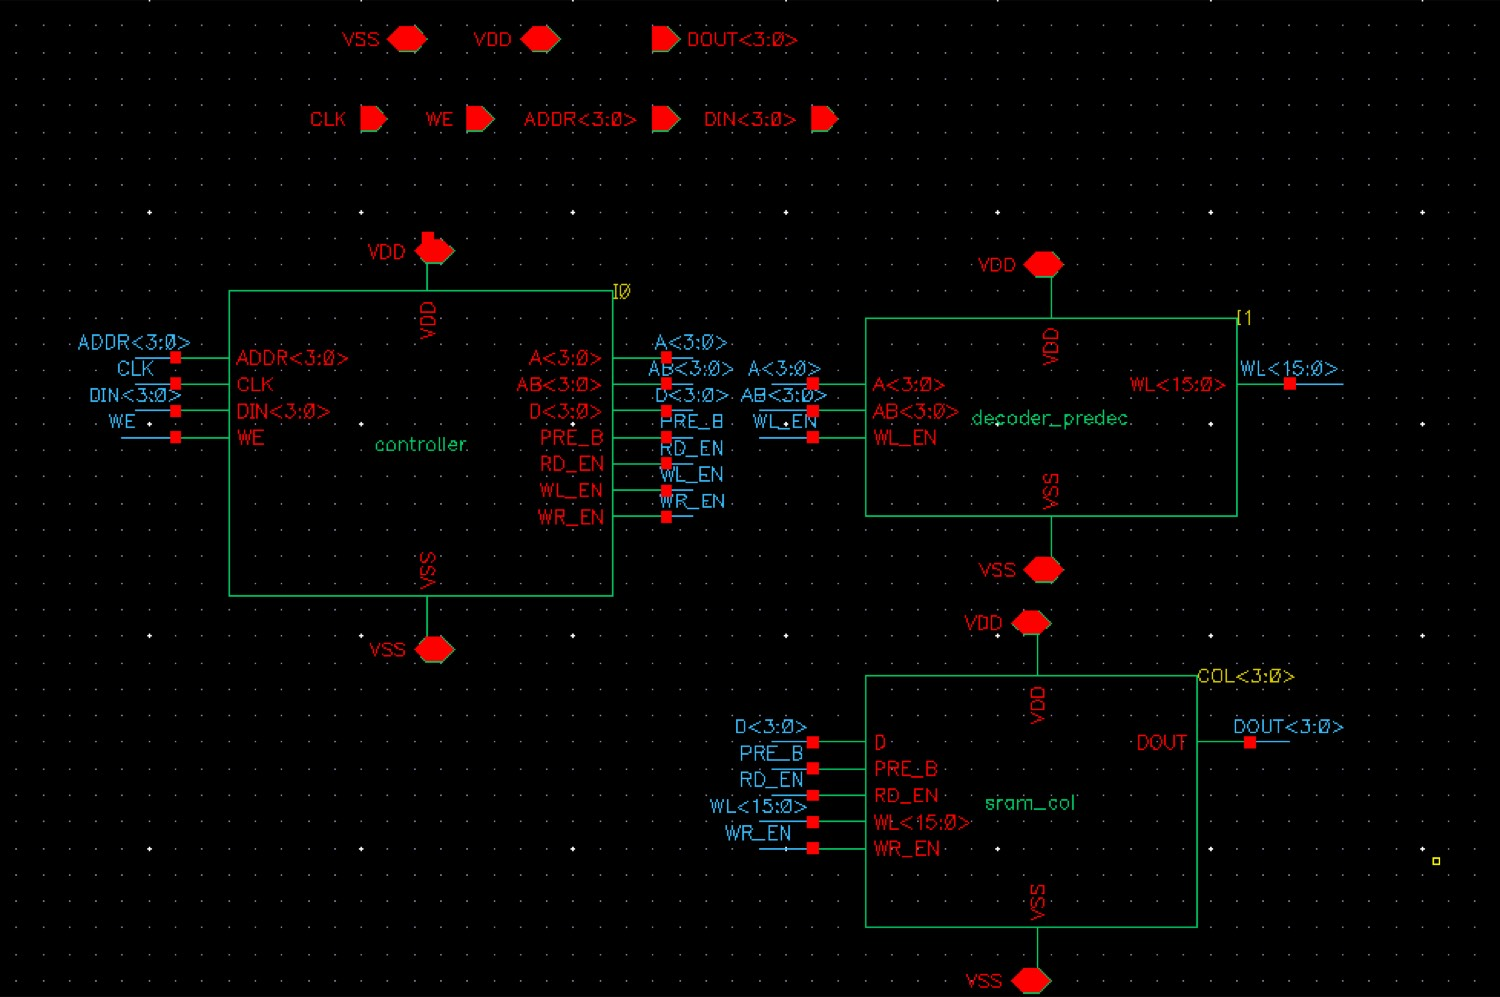
\includegraphics[width=.72\linewidth]{sram_macro_schematic}
\caption{\code{sram\_macro}: controller, \code{decoder\_predec} and four \code{sram\_col} instances. Ports CLK, WE, ADDR$\langle3{:}0\rangle$, DIN$\langle3{:}0\rangle$, DOUT$\langle3{:}0\rangle$ match the handout.}\end{figure}

%==============================================================
\section{Array layout and extraction (2.1)}
The array \code{6t\_sram\_64b} is 16 rows by 4 columns of the Part 1 cell, mirrored so neighbours share bitline contacts and the VDD/VSS rails. Pitch is the Part 1 PR box: $0.72$ $\mu$m along the wordline (four columns) and $0.54$ $\mu$m along the bitline (sixteen rows), so the tile is $2.88\times8.64$ $\mu$m $=24.9$ $\mu$m$^2$.

Pegasus 23.20 DRC of the array is clean: 0 results in 0 of 374 checks. Pegasus LVS of the tiled cell is ISL clean with comparison match (\code{6t\_sram\_final\_design}). The array schematic is 64 instances of that cell; abutment joins matching BL, BLB, WL, VDD and VSS pins, so the layout connectivity is the cell LVS plus those shared rails.

\begin{figure}[H]\centering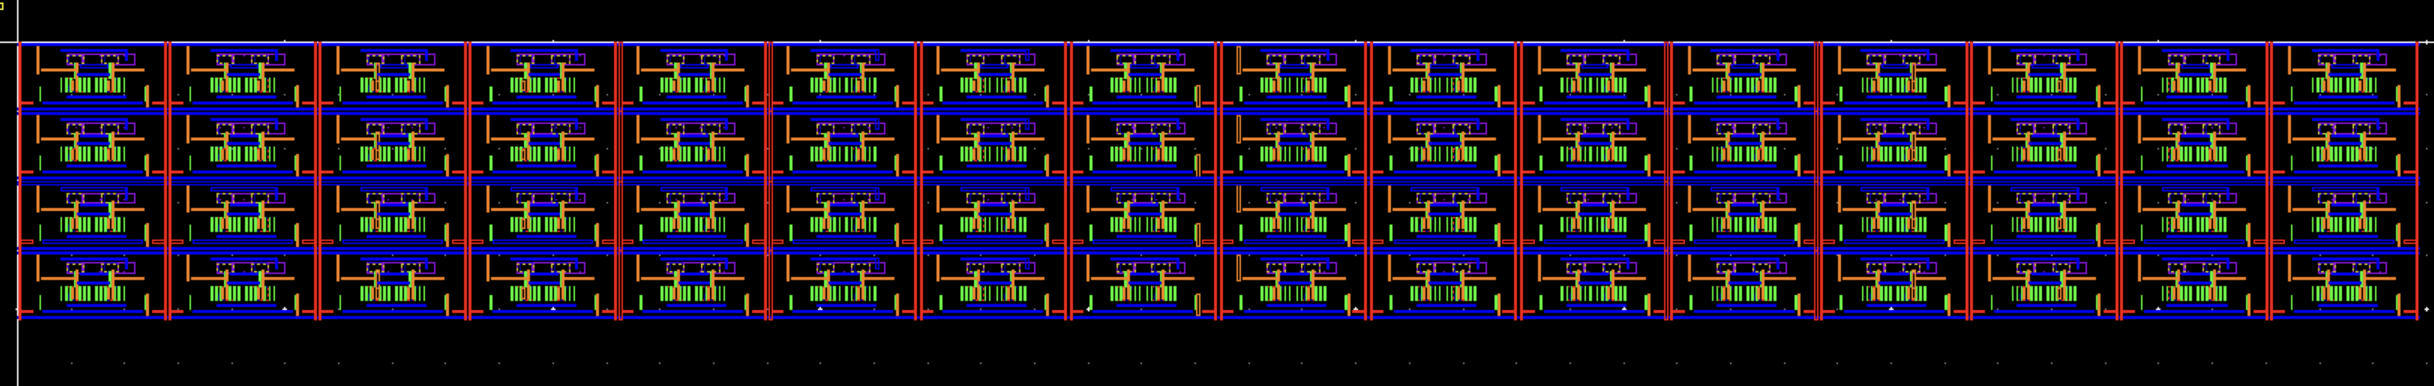
\includegraphics[width=\linewidth]{64b_full}
\caption{Tiled 16$\times$4 array \code{6t\_sram\_64b} (64 bitcells). PR boundary $2.88\times8.64$ $\mu$m.}\end{figure}
\begin{figure}[H]\centering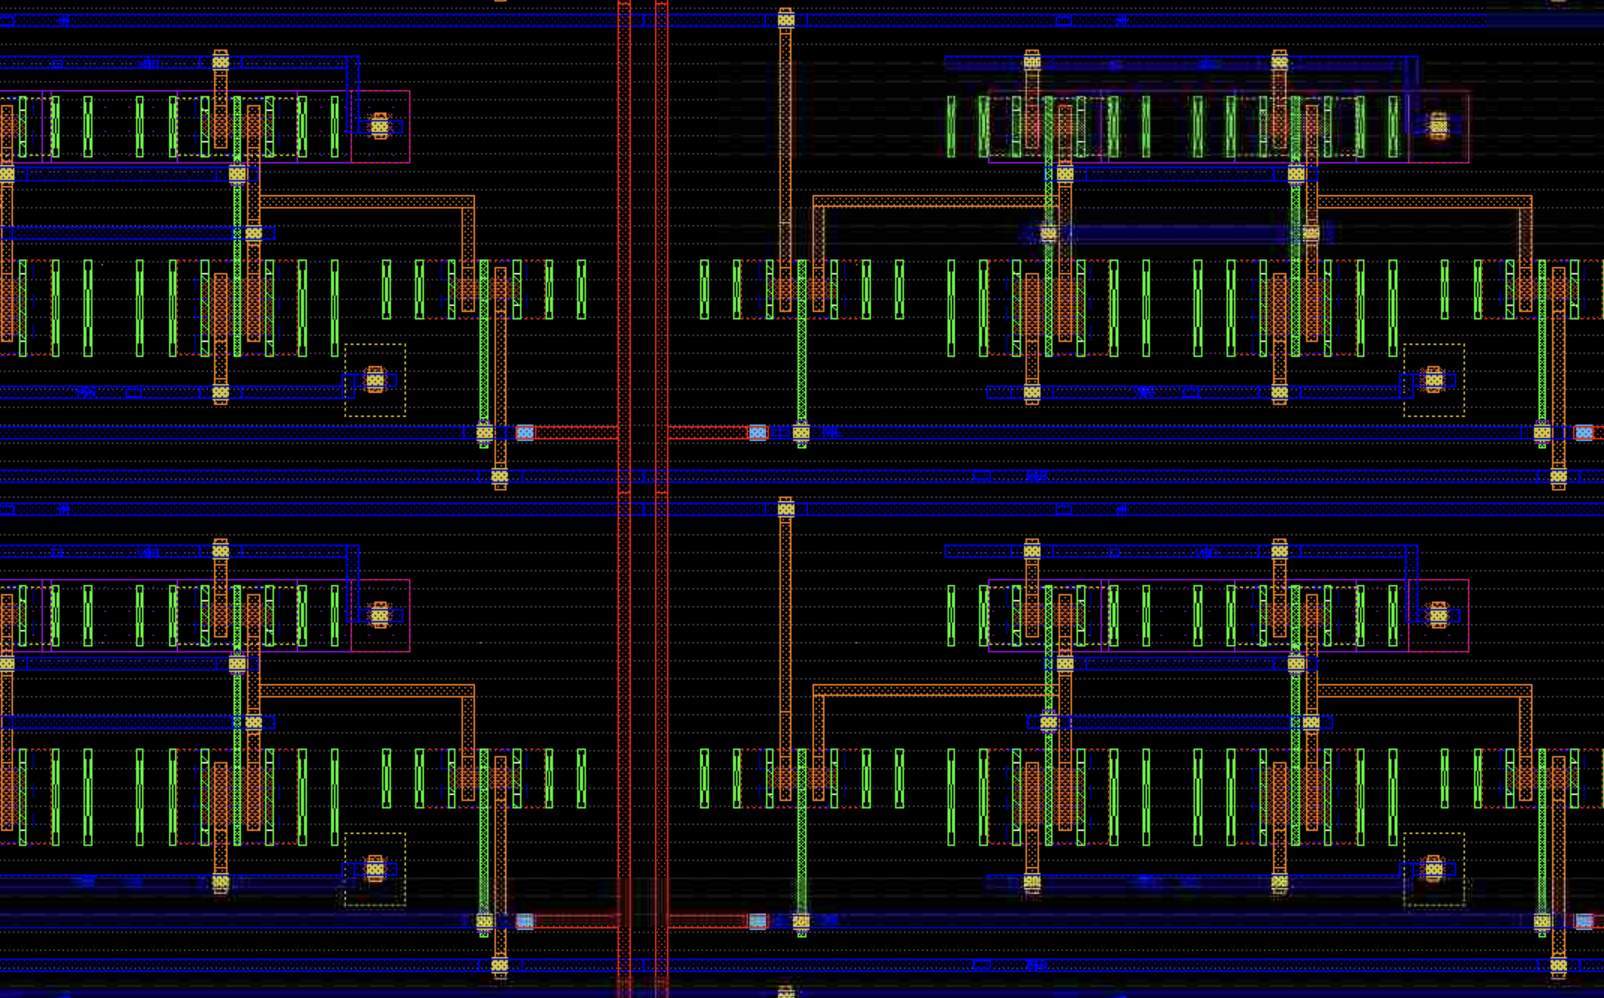
\includegraphics[width=.92\linewidth]{64b_layout_closeup}
\caption{Four mirrored cells sharing the centre bitline contacts and the horizontal supply rails.}\end{figure}
\begin{figure}[H]\centering
\begin{subfigure}{.48\linewidth}\centering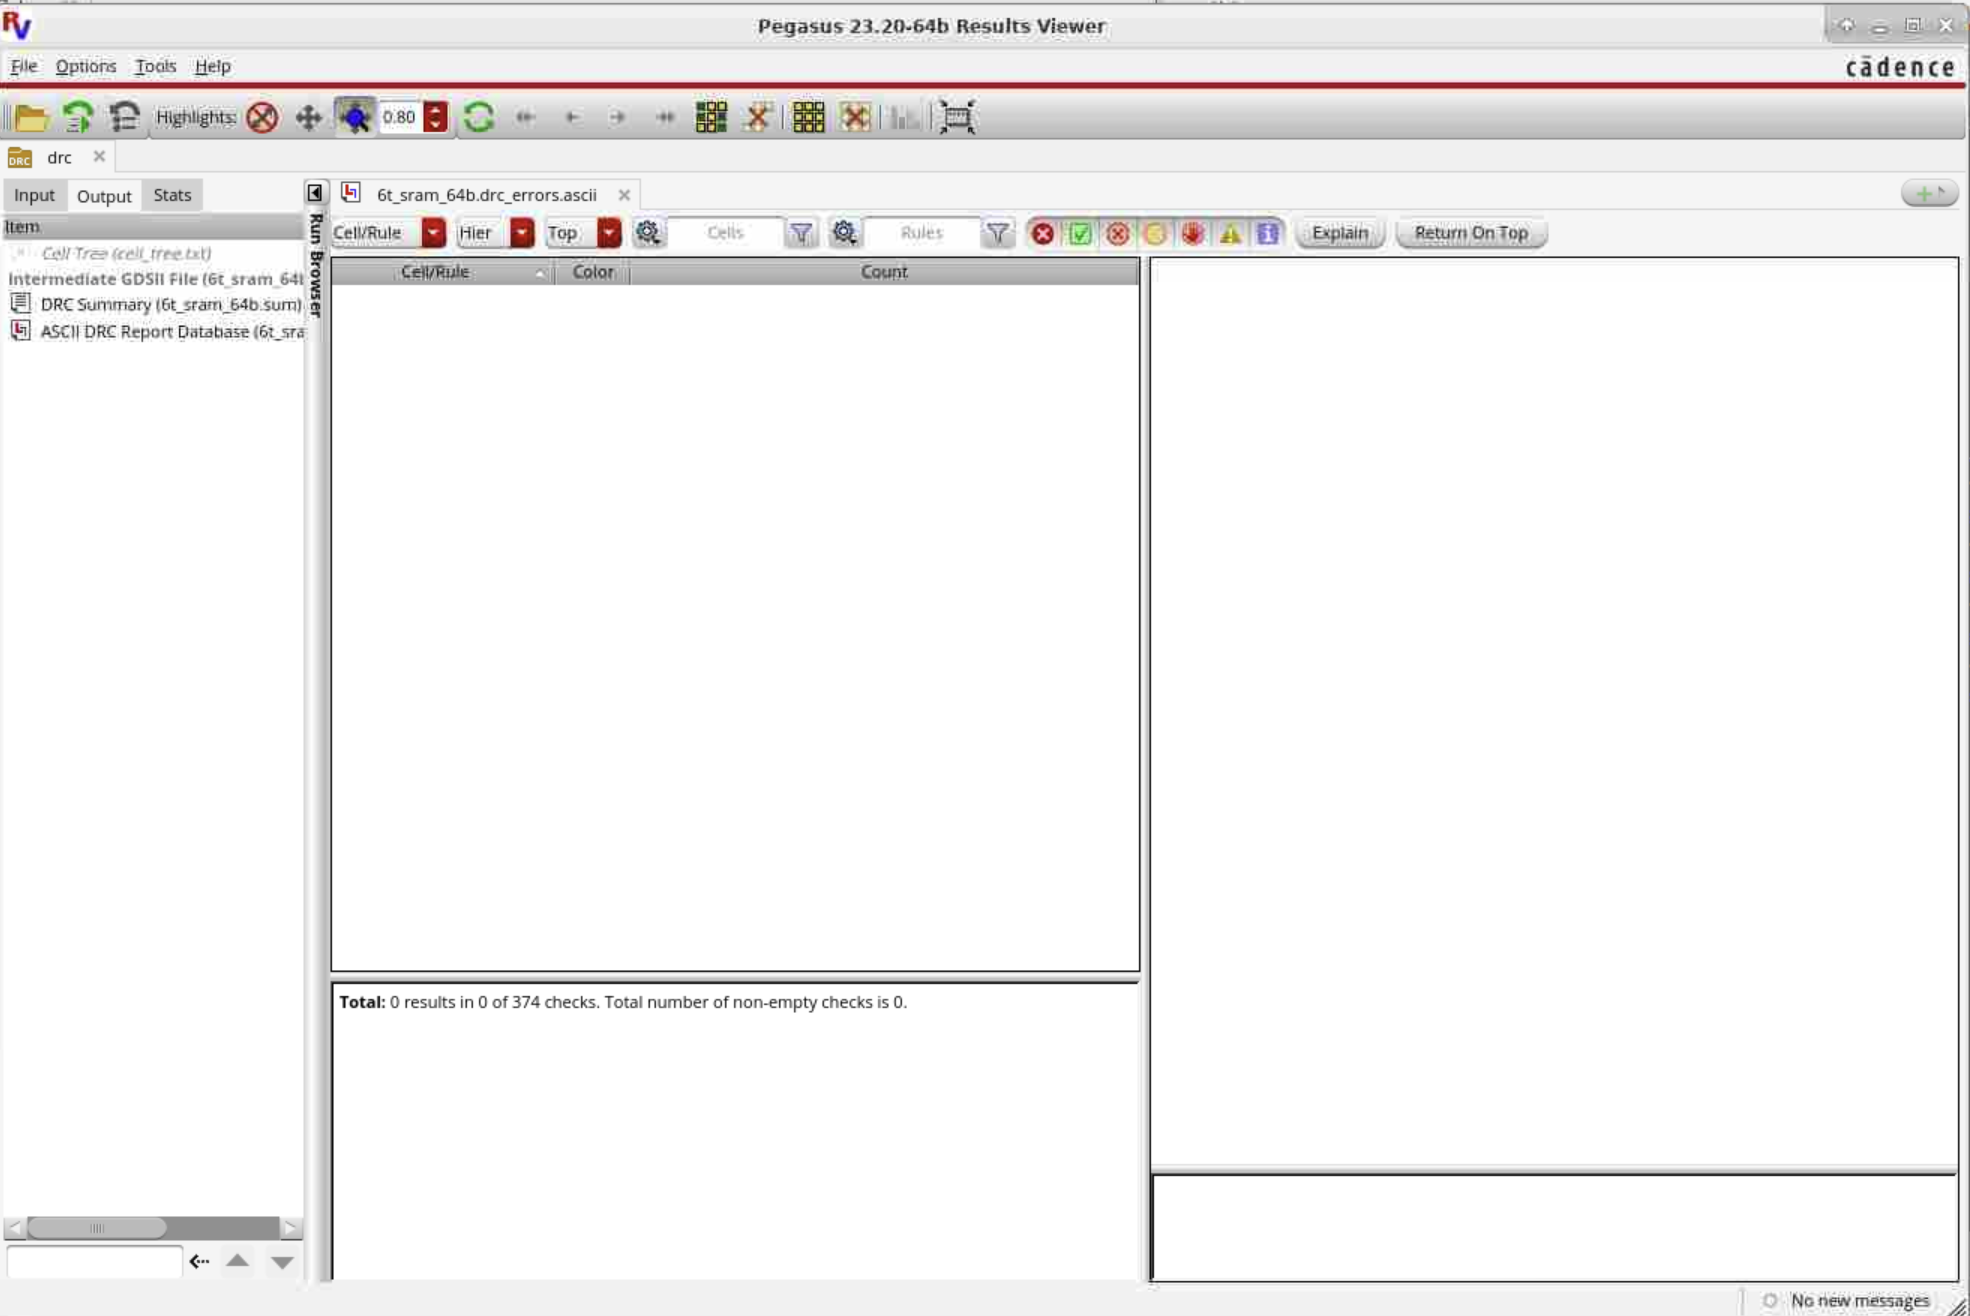
\includegraphics[width=\linewidth]{drc_64b}
\caption{Array DRC: 0 of 374.}\end{subfigure}\hfill
\begin{subfigure}{.48\linewidth}\centering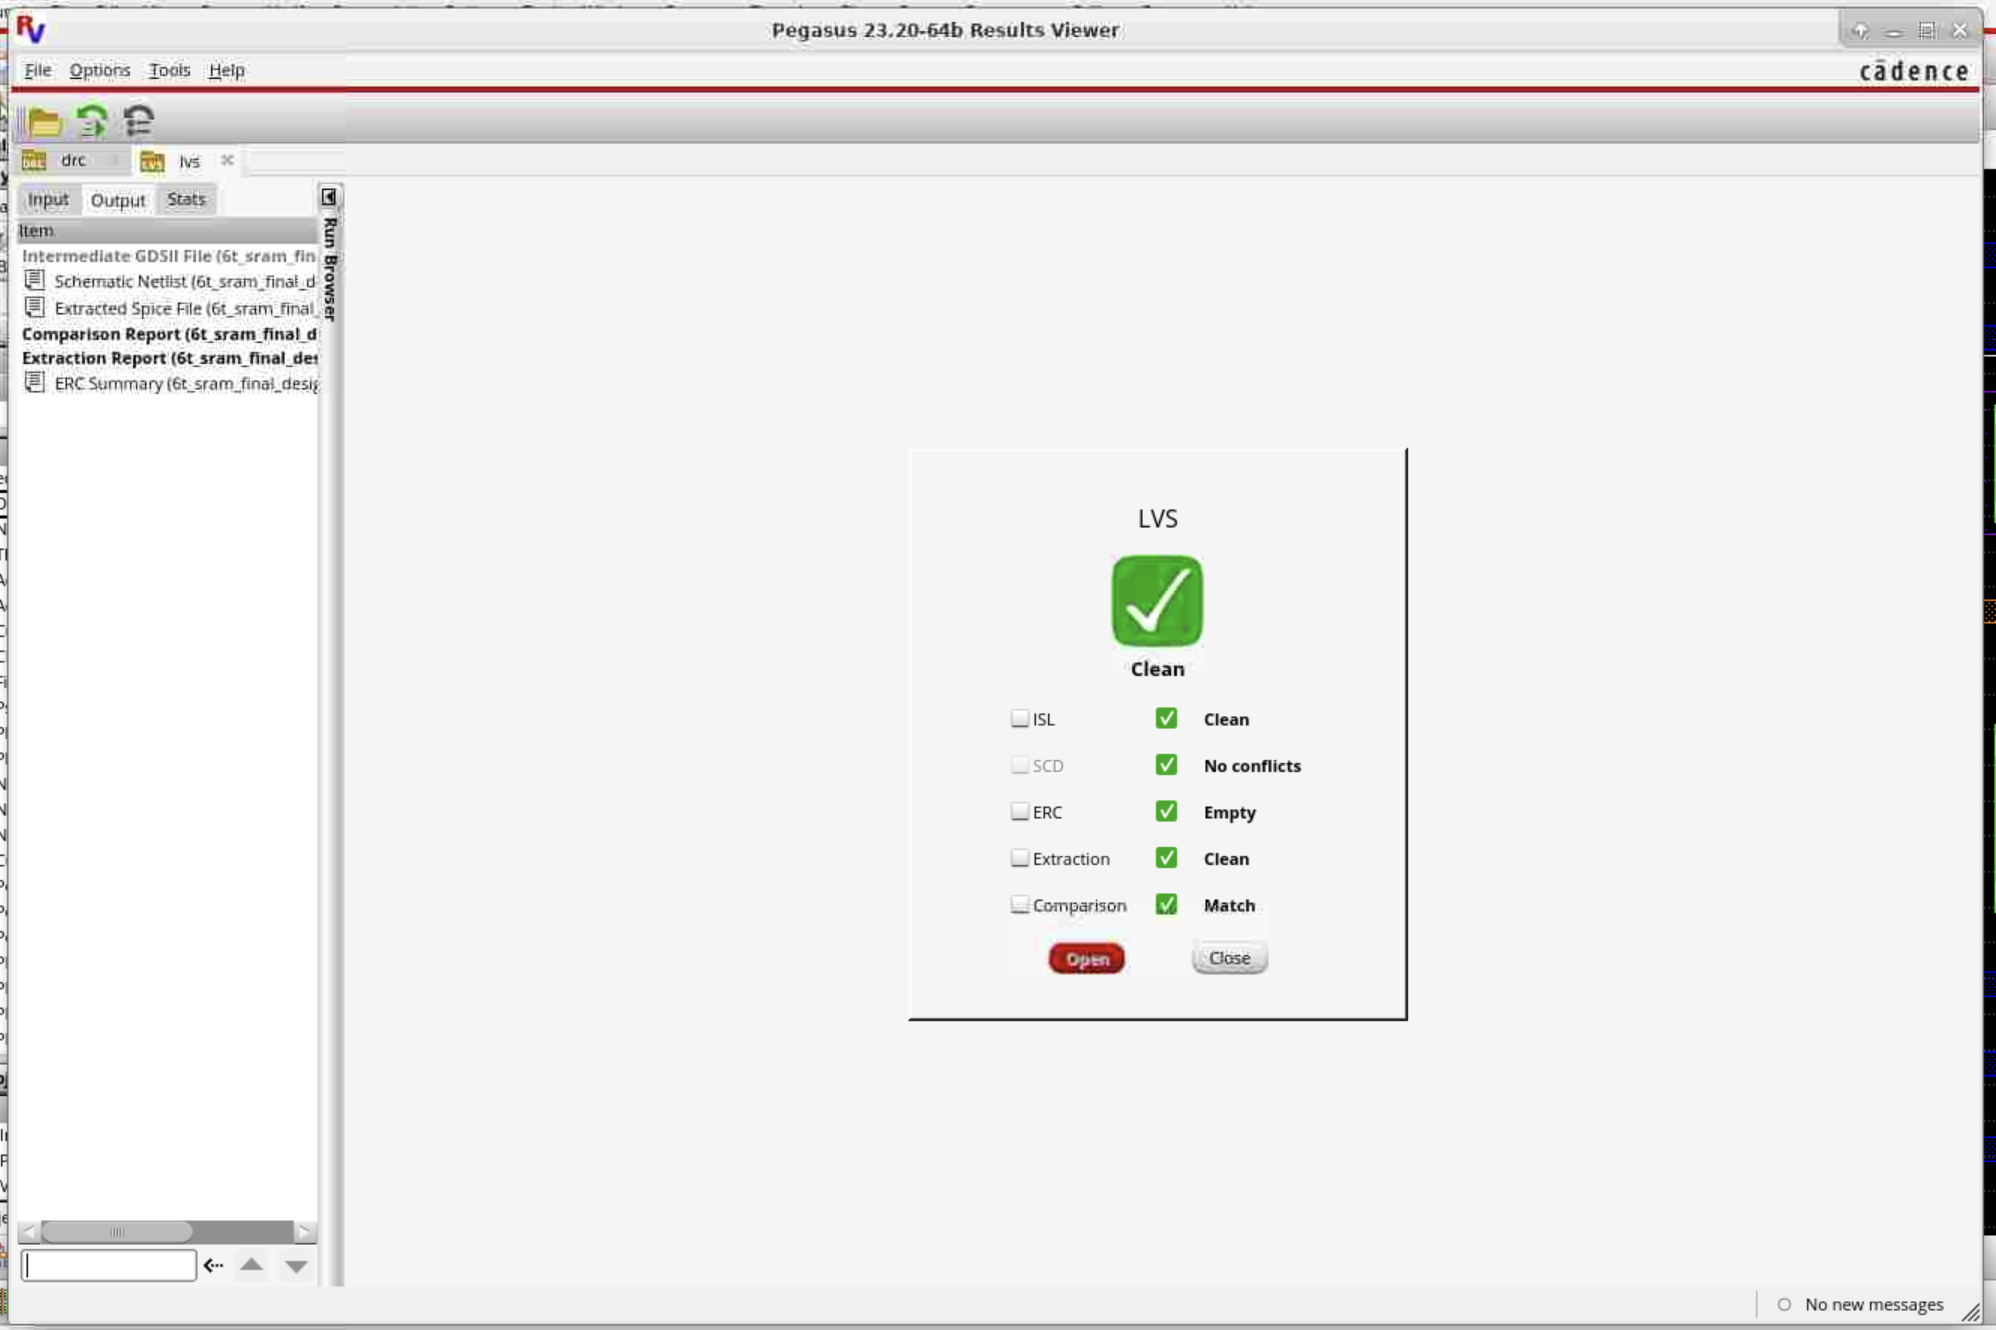
\includegraphics[width=\linewidth]{lvs_pass}
\caption{Cell LVS: ISL clean.}\end{subfigure}
\caption{Pegasus 23.20: DRC of \code{6t\_sram\_64b} and LVS of the instance cell \code{6t\_sram\_final\_design}.}\end{figure}

Quantus 23.1.2 on the Part 1 cell (typical, $25^\circ$C, \code{rc\_decoupled}) wrote \code{av\_extracted}: 132~$R$, 97~$C$, 4~\code{n1svt} $+$ 2~\code{p1svt}. All-Parasitics sums (decoupled $+$ coupled $+$ self $C$) are the net parasitics on each pin.

\begin{figure}[H]\centering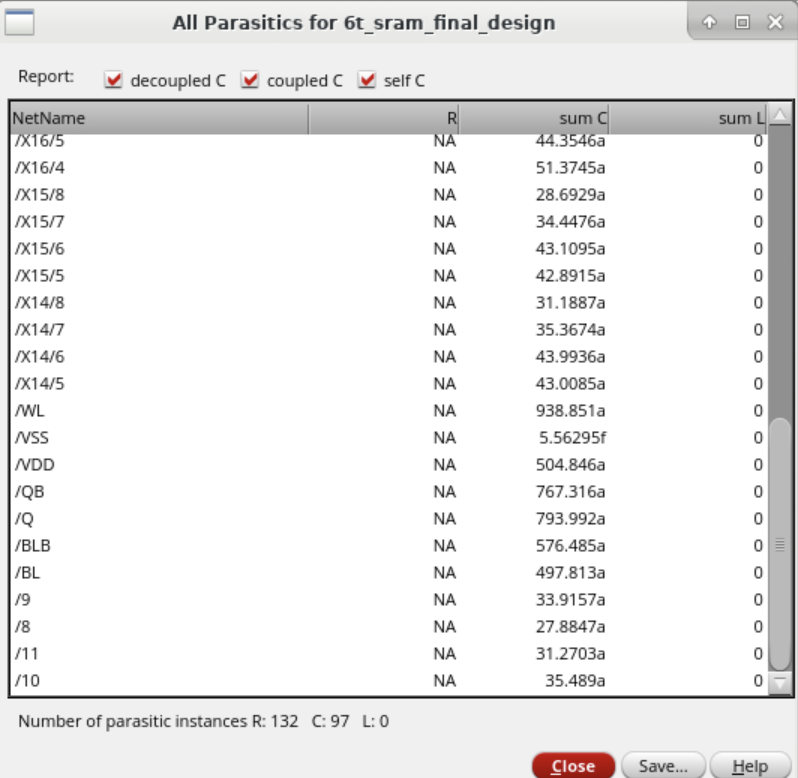
\includegraphics[width=.72\linewidth]{parasitics_extraction}
\caption{Quantus All Parasitics for \code{6t\_sram\_final\_design}: $C_{BL}=497.8$ aF, $C_{BLB}=576.5$ aF, $C_{WL}=938.9$ aF.}\end{figure}

A column of 16 cells presents $16\times$ the cell bitline net; a wordline of 4 cells presents $4\times$ the cell wordline net. Adding $0.62$ fF of M1/M2 array wire (the term used on the macro bench) gives the extracted column and row loads in Table~\ref{tab:cap}. Those values are the $C_{BL}$ and $C_{WL}$ used for decoder effort, the read-pulse calculation, and the $+20\%$ recovery in Sections~\ref{sec:le}--\ref{sec:ctrl}.

\begin{table}[H]\centering
\caption{Bitline and wordline capacitance from Part 1 Quantus, scaled to the 16$\times$4 array.}\label{tab:cap}
\begin{tabular}{@{}lcccc@{}}\toprule Quantity & Part 1 cell & $\times$ cells & $16\times$/$4\times$ & $+$ $0.62$ fF wire\\\midrule
$C_{BL}$  & 497.8 aF & 16 & 7.97 fF & $\mathbf{8.59}$ fF\\
$C_{BLB}$ & 576.5 aF & 16 & 9.22 fF & $\mathbf{9.84}$ fF\\
$C_{WL}$  & 938.9 aF & 4  & 3.76 fF & $\mathbf{4.38}$ fF\\\bottomrule\end{tabular}
\end{table}

Column unit tests were closed at $3.5$ fF and the decoder at $0.5$ fF per wordline (the loads on those benches). Table~\ref{tab:scale} carries every measured delay to the extracted $8.59$ fF and to $+20\%$ of extracted ($10.3$ fF) with the $3.5\to4.2$ fF slope for writes and $C$-proportional scaling for the bitline fall and precharge.

\begin{table}[H]\centering\small
\caption{Column delays at the test load, at $+20\%$ of the test load, and at the extracted array $C_{BL}$.}\label{tab:scale}
\begin{tabular}{@{}lcccc@{}}\toprule Quantity & $3.5$ fF & $4.2$ fF & $8.59$ fF & $10.3$ fF\\\midrule
Write, nfin 8 (ps) & $96$ meas. & $102$ meas. & $140$ & $154$\\
$t_{blb}$ to $V_M$ (ps) & $83$ meas. & $100$ & $204$ & $245$\\
$t_{BL}=C\Delta V/I_{\rm cell}$ (ps) & $59$ & $71$ & $146$ & $175$\\
Precharge restore (ps) & $124$ & $149$ & $304$ & $364$\\\bottomrule\end{tabular}
\end{table}

\textbf{Area} (Part 1 convention: $D=28$, $W_{\rm fin}=0.048$ $\mu$m, $L=18$ nm, $0.0242$ $\mu$m$^2$ per fin):
\begin{center}\small\begin{tabular}{lrrr}\toprule Block & Instances & Fins & Area, $\mu$m$^2$\\\midrule
Array, $2.88\times8.64$ $\mu$m (\code{6t\_sram\_64b}) & 64 & -- & 24.9\\
Row decoder & 1 & 520 & 12.6\\
Controller (23 \code{inv\_u}, 9 latches, 4 \code{inv\_2x}, 3 \code{nand2\_u}) & 1 & 426 & 10.3\\
Write drivers / precharge / read paths / latches & 4 each & 144 / 24 / 16 / 96 & 3.5 / 0.58 / 0.39 / 2.3\\\midrule
Periphery $=D\sum W_iL_i$ & & 1226 & 29.7\\
Macro total & & & \textbf{54.6}\\\bottomrule\end{tabular}\end{center}
The array term is the tiled PR-boundary area. The periphery is $D\sum W_iL_i$. Testbench buffers are excluded.

%==============================================================
\section{Row decoder and wordline timing (2.2)}
\subsection{Gates and sizes}
Every gate is built from \code{inv\_u} (PMOS 4 fins, NMOS 2 fins, $L=18$ nm). \code{nand3\_u} keeps that pull-down: NMOS 6 fins, PMOS 4. \code{nand2\_u} is 2 fins on every device (half of \code{inv\_u}; logical effort unchanged). \code{inv\_2x} is 8/4; \code{inv\_drv} is 6/3.
\begin{figure}[H]\centering
\begin{subfigure}{.19\linewidth}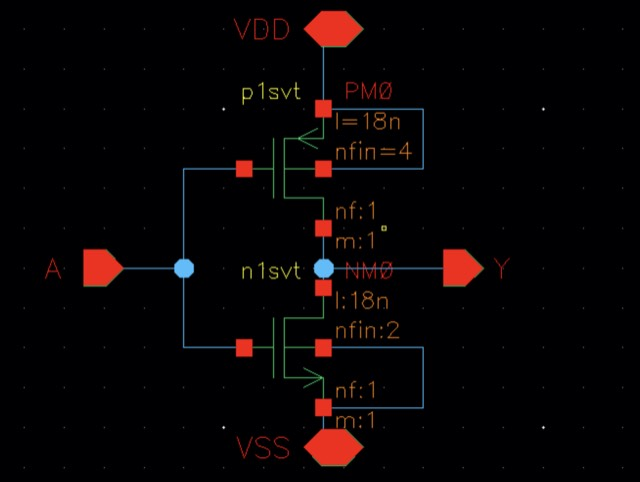
\includegraphics[width=\linewidth]{inv_u_schematic}\caption{\code{inv\_u}}\end{subfigure}\hfill
\begin{subfigure}{.19\linewidth}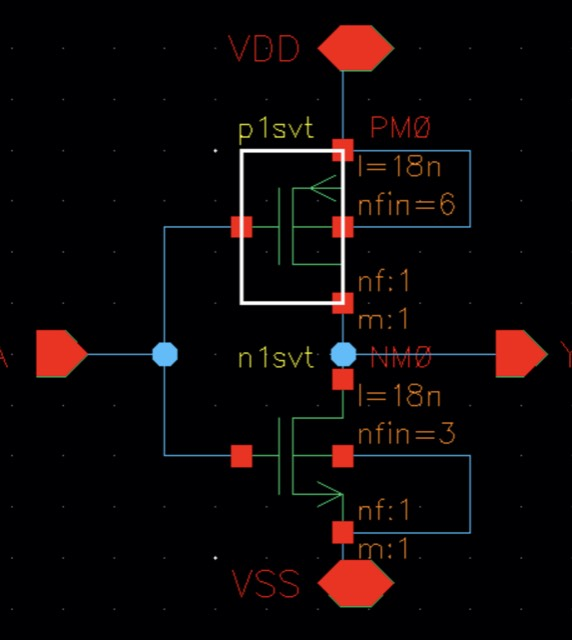
\includegraphics[width=\linewidth]{inv_drv_schematic}\caption{\code{inv\_drv}}\end{subfigure}\hfill
\begin{subfigure}{.19\linewidth}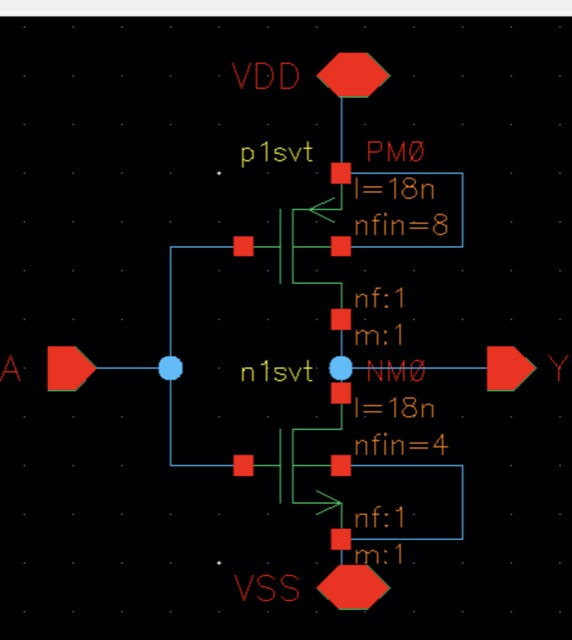
\includegraphics[width=\linewidth]{inv_2x_schematic}\caption{\code{inv\_2x}}\end{subfigure}\hfill
\begin{subfigure}{.19\linewidth}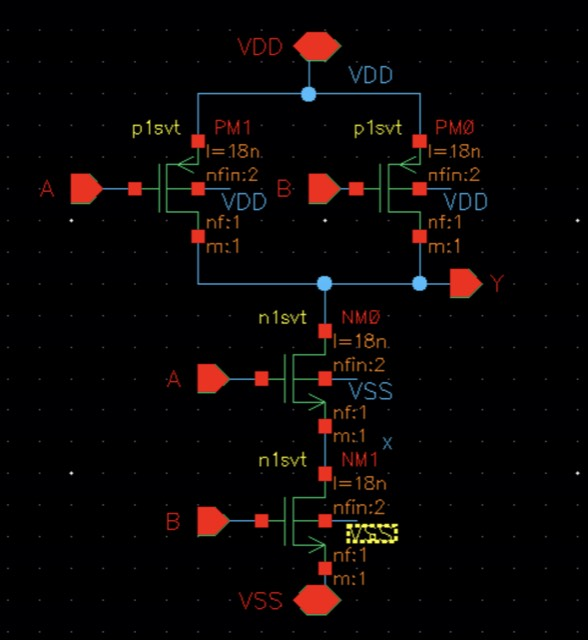
\includegraphics[width=\linewidth]{nand2_u_schematic}\caption{\code{nand2\_u}}\end{subfigure}\hfill
\begin{subfigure}{.19\linewidth}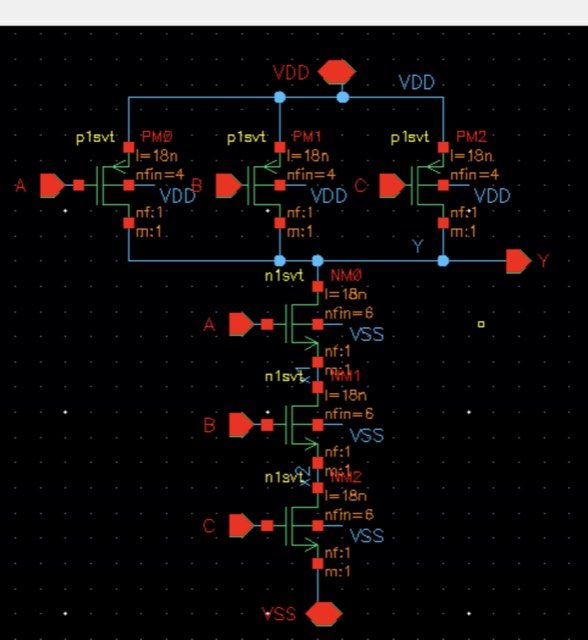
\includegraphics[width=\linewidth]{nand3_u_schematic}\caption{\code{nand3\_u}}\end{subfigure}
\caption{Decoder gates, fins per device, $L=18$ nm.}\end{figure}

\subsection{Chosen implementation: 2-2 predecode}
PA$\langle j\rangle=$ WL\_EN$\cdot(A_{1:0}=j)$ from \code{nand3\_u}+\code{inv\_2x}; PB$\langle m\rangle=(A_{3:2}=m)$ from \code{nand2\_u}+\code{inv\_2x}; WL$\langle4m+j\rangle=$ PA$\langle j\rangle\cdot$PB$\langle m\rangle$ from \code{nand2\_u}+\code{inv\_drv}. Each literal reaches two predecode gates and each predecode output drives four rows, so $B=8$ as the handout requires.
\begin{figure}[H]\centering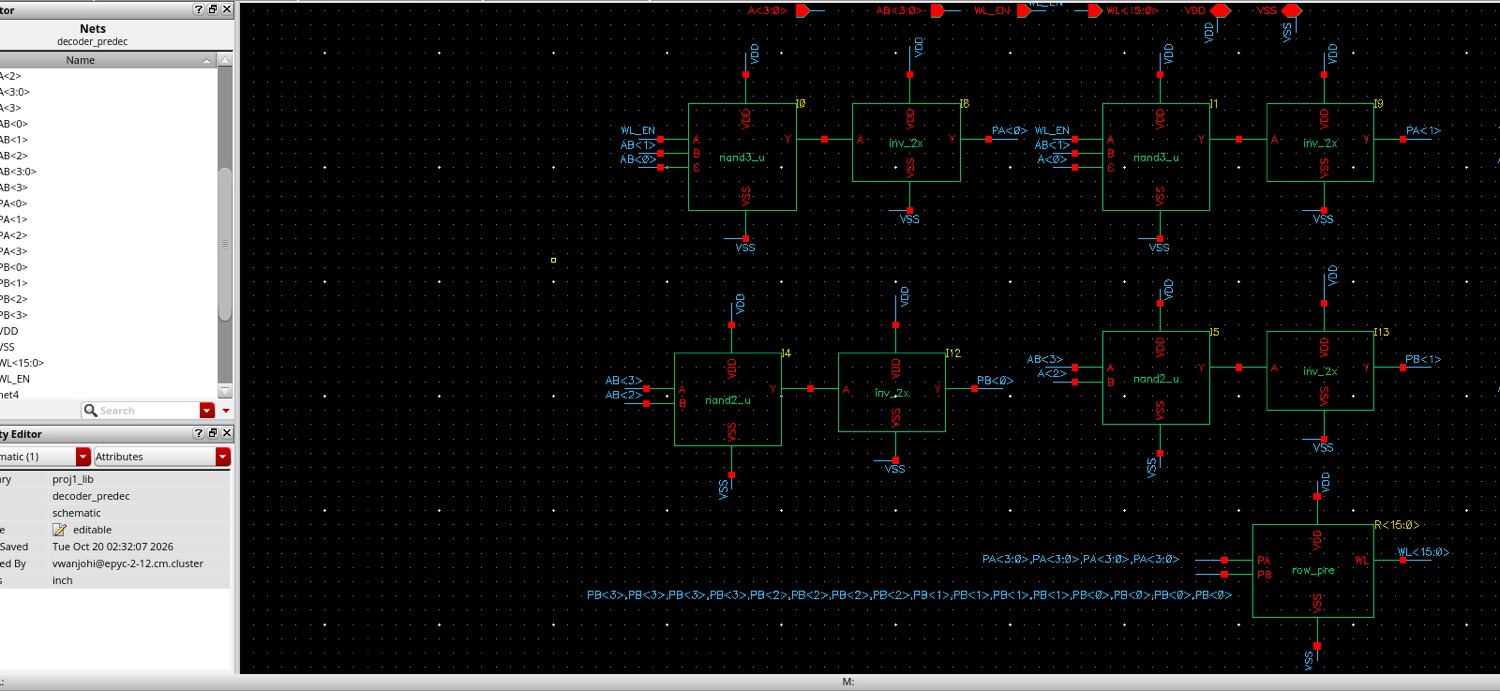
\includegraphics[width=.92\linewidth]{decoder_predec_schematic}
\caption{\code{decoder\_predec}: PA (top), PB (middle) and sixteen \code{row\_pre} instances.}\end{figure}
\begin{figure}[H]\centering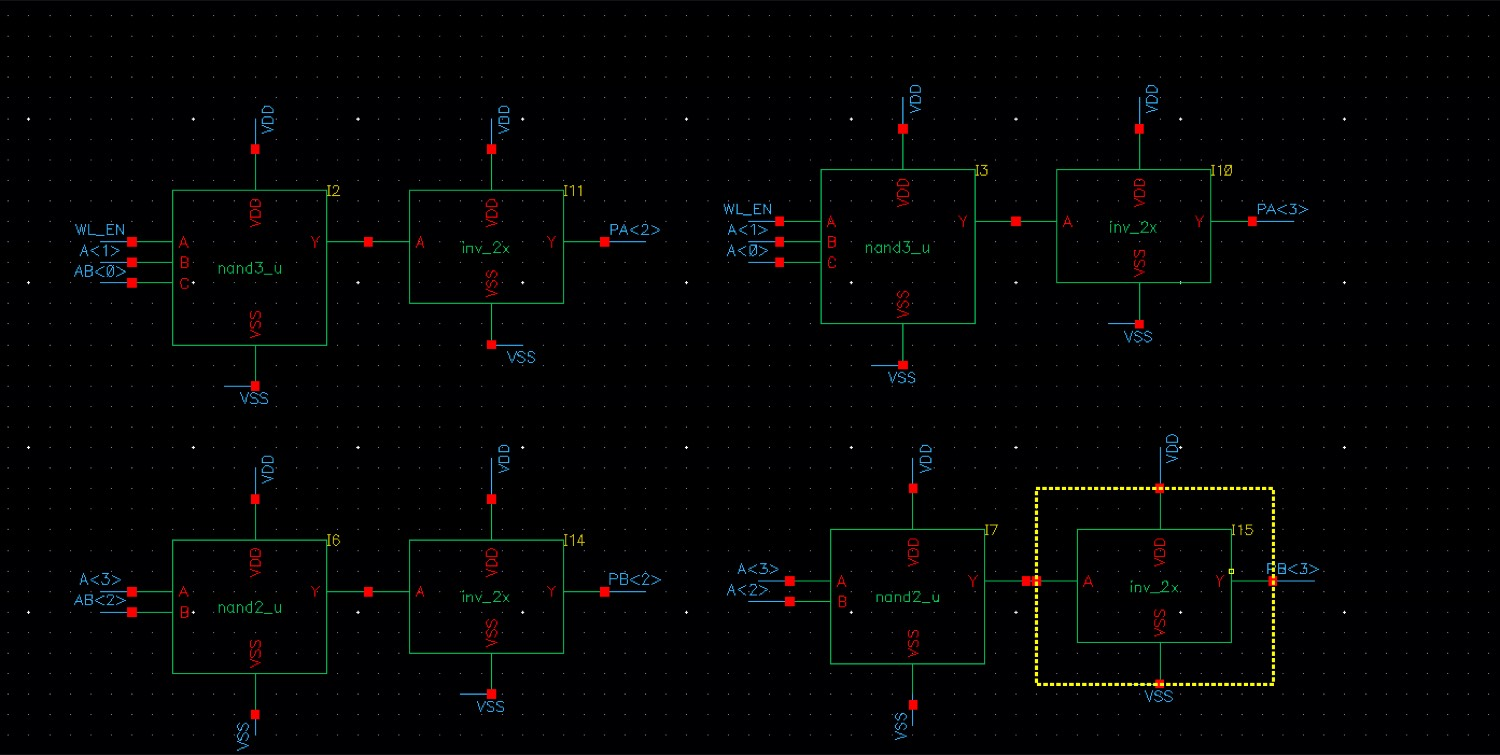
\includegraphics[width=.78\linewidth]{decoder_predec_gate_detail}
\caption{One PA NAND3, one PB NAND2 and one row NAND2+driver, as drawn.}\end{figure}

\subsection{Logical effort from an address input (2.2a)}\label{sec:le}
FO4 of \code{inv\_u} is $52.6$ ps ($t_{pHL}=54.7$ ps, $t_{pLH}=50.6$ ps), so $\tau=10.5$ ps. Gate capacitance $\approx20$ aF/fin. $p_{\rm INV}=1$, $p_{\rm NAND2}=2$, $p_{\rm NAND3}=3$, $p_{\rm NAND4}=4$. Electrical effort uses $C_{WL}=4.38$ fF (Table~\ref{tab:cap}) and, for the decoder bench, $0.5$ fF.

The path from ADDR to WL is four stages. $A_0$ and $A_1$ (and WL\_EN) enter \code{nand3\_u}: NAND3--INV--NAND2--INV, $G=\tfrac53\cdot1\cdot\tfrac43\cdot1=\tfrac{20}{9}=2.22$, $C_{in}=10$ fins $=200$ aF. $A_2$ and $A_3$ enter \code{nand2\_u}: NAND2--INV--NAND2--INV, $G=\tfrac43\cdot1\cdot\tfrac43\cdot1=\tfrac{16}{9}=1.78$, $C_{in}=4$ fins $=80$ aF. In both cases each literal fans out to two predecode gates and each predecode output to four rows, $B=8$.

Optimal stage count $\hat N=\log_4 F$ with $F=GBH$. Four stages is the right count for the NAND3 path at the extracted $C_{WL}$ ($\hat N=4.3$). The NAND2 address path has a smaller $C_{in}$ and a larger $H$; $\hat N=4.8$, so four stages is slightly short of the effort-4 target and that path is the slower of the two address bits.

\begin{table}[H]\centering\small
\caption{Logical effort, address input $\to$ WL, 2-2 predecode.}\label{tab:leA}
\begin{tabular}{@{}lcccccc@{}}\toprule Path & $C_{WL}$ & $H$ & $F$ & $\hat N$ & $f$ & $D$\\\midrule
$A_{1:0}$ / WL\_EN & $0.5$ fF & $2.5$ & $44$ & $2.7$ & $2.6$ & $17.3\,\tau=182$ ps\\
$A_{1:0}$ / WL\_EN & $4.38$ fF & $21.9$ & $389$ & $4.3$ & $4.4$ & $24.8\,\tau=260$ ps\\
$A_{3:2}$ & $0.5$ fF & $6.3$ & $89$ & $3.2$ & $3.1$ & $18.3\,\tau=192$ ps\\
$A_{3:2}$ & $4.38$ fF & $54.8$ & $779$ & $4.8$ & $5.3$ & $27.1\,\tau=285$ ps\\\bottomrule\end{tabular}
\end{table}
$N=4$ is kept: adding a fifth inverter would cost a stage of parasitic delay for a modest drop in $f$ on the $A_{3:2}$ path, and the measured WL\_EN$\to$WL delay is already $97$ ps.

\subsection{Second implementation: flat NAND4 (2.2b)}
The alternative is one 4-input NAND of the address literals plus \code{inv\_drv} on every row, with WL\_EN as a fifth stacked NMOS (NAND5, $g=\tfrac73$). Two stages. $G=\tfrac73$, $B=8$, $C_{in}\approx8$ fins $=160$ aF.

At $C_{WL}=0.5$ fF: $H=3.1$, $F=58$, $f=7.6$, $P=6$, $D=21.2\,\tau\approx223$ ps.
At $C_{WL}=4.38$ fF: $H=27.4$, $F=511$, $f=22.6$, $D=51\,\tau\approx540$ ps.

The 2-2 path keeps stage effort near 4 once $C_{WL}$ is the extracted net; the flat path is effort-starved at two stages. Only A was built. Applying the measured/predicted ratio of A ($97/182=0.53$) to B gives the schematic delays in the last column of Table~\ref{tab:le}.

\begin{table}[H]\centering
\caption{Predicted WL\_EN$\to$WL delay versus the measured 2-2 predecode. The last column scales B by A's $97/182$ ratio.}\label{tab:le}
\begin{tabular}{@{}lcccc@{}}\toprule Implementation & Predict, $0.5$ fF & Predict, $4.38$ fF & Measured, $0.5$ fF & Scaled, $0.5$ fF\\\midrule
2-2 predecode (A) & 182 ps & 260 ps & \textbf{97 ps} & 97 ps\\
Flat NAND4+driver (B) & 223 ps & 540 ps & --- & 119 ps\\\bottomrule\end{tabular}
\end{table}
A is faster at both loads. The $0.5$ fF prediction is conservative ($1.9\times$ the measured $97$ ps); the extracted $C_{WL}$ raises the prediction to $260$ ps, still inside the $500$ ps clock high at $1$ ns and inside the $345$ ps high at $T_{CLK,\min}$.

\subsection{Measured decoder delay}
\code{tb\_dec\_pre}, $0.5$ fF per wordline, WL\_EN $300$ ps with $20$ ps edges, static address. WL\_EN$\to$WL is $97.4$ ps rising and $101$ ps falling at every address (WL\_EN always enters the same \code{nand3\_u} pin). Peak of the summed wordlines is $824$ mV at all 16 addresses: exactly one row high ($<1$ V) and it reaches high ($>0.72$ V). \code{wl\_idx} (row index weighted by wordline peak over $0.824$ V) returns the selected row:
\begin{center}\scriptsize\setlength{\tabcolsep}{2.8pt}\begin{tabular}{l|cccccccccccccccc}\toprule Address & 0&1&2&3&4&5&6&7&8&9&10&11&12&13&14&15\\\midrule
\code{wl\_idx} & 0.06&1.06&2.06&3.06&4.03&5.04&6.04&7.04&8.01&9.01&10.01&11.01&11.98&12.98&13.99&14.99\\\bottomrule\end{tabular}\end{center}
Each value is distinct and within $0.07$ of its row. Offsets are $\approx2$ mV coupling on rows sharing PA$\langle0\rangle$.
\begin{figure}[H]\centering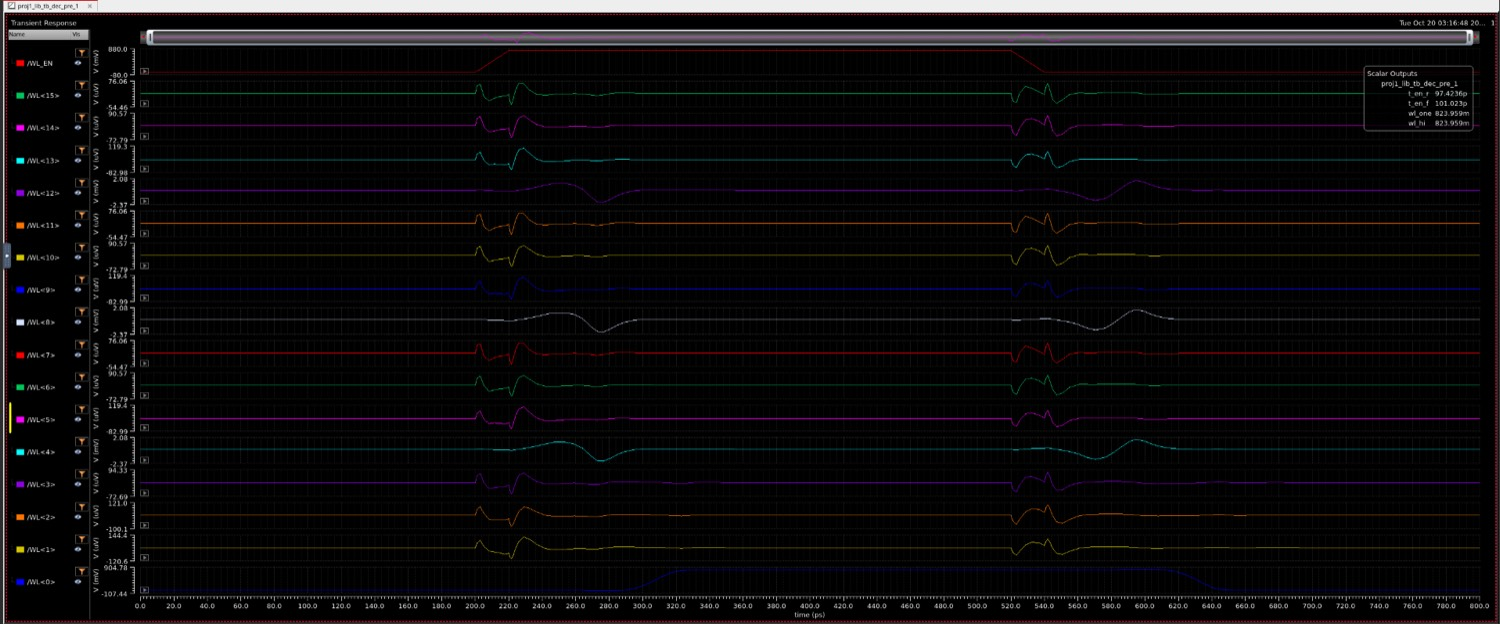
\includegraphics[width=.82\linewidth]{tb_dec_pre_tran_addr0}
\caption{Address 0: only WL$\langle0\rangle$ rises; unselected rows stay within $2$ mV.}\end{figure}
\begin{figure}[H]\centering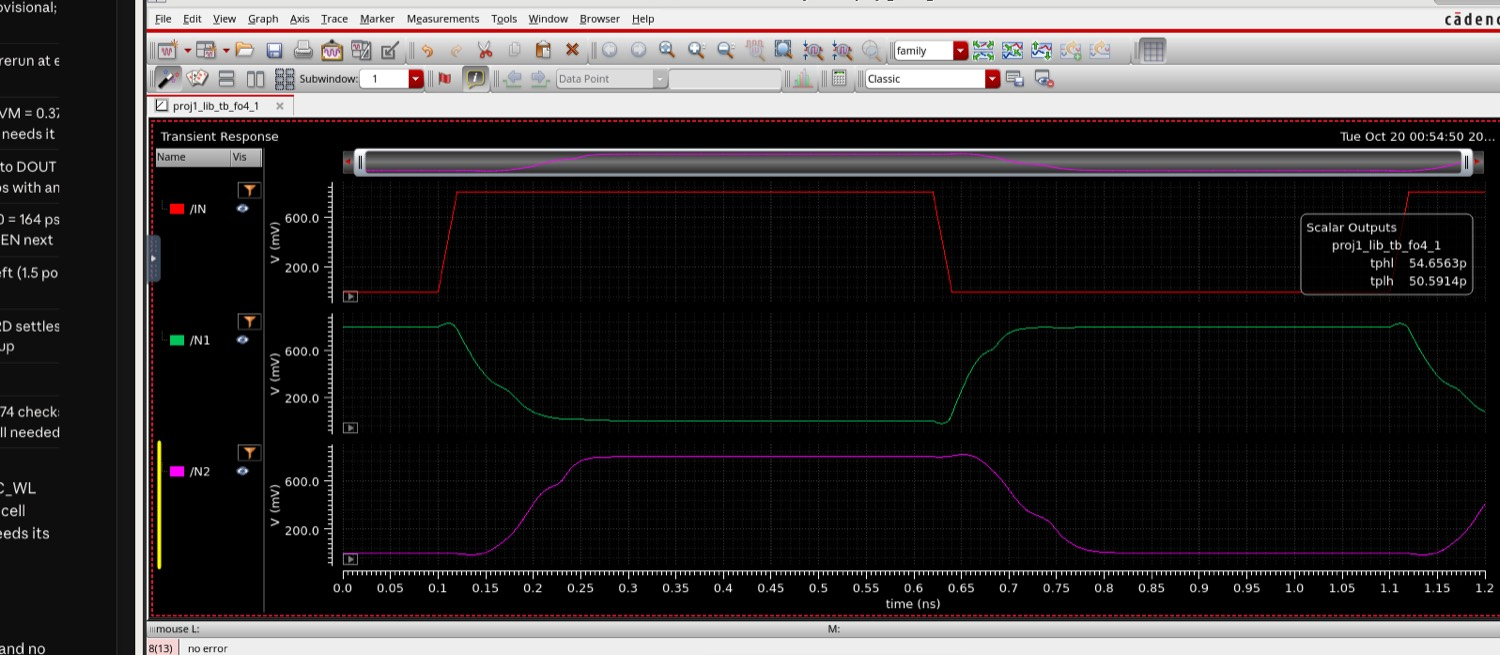
\includegraphics[width=.7\linewidth]{tb_fo4_tran}
\caption{\code{tb\_fo4}: IN, N1, N2 of an \code{inv\_u} chain. FO4 $=53$ ps.}\end{figure}

\subsection{Wordline pulse width (2.2c)}
The read needs the bitline to fall $\Delta V=V_{DD}-V_M=0.424$ V through the cell current $I_{\rm cell}=25$ $\mu$A (Part 1, $0.8$ V):
\begin{equation}
t_{BL}=\frac{C_{BL}\,\Delta V}{I_{\rm cell}}.
\end{equation}
At the column-test load $C_{BL}=3.5$ fF this is $59$ ps. The measured BLB time to $V_M$ is $83$ ps; the extra $24$ ps is the drop in $I_{\rm cell}$ as $V_{DS}$ of the pass-gate falls. At the extracted $C_{BL}=8.59$ fF the same formula gives $146$ ps, and $C$-scaling of the measured $83$ ps gives $204$ ps.

\begin{center}\small\begin{tabular}{lll}\toprule Quantity & Value & Source\\\midrule
$t_{BL}$, $3.5$ fF, $C\Delta V/I_{\rm cell}$ & 59 ps & $I_{\rm cell}=25$ $\mu$A, $\Delta V=0.424$ V\\
$t_{blb}$ measured & 83 ps & read-column test, $3.5$ fF\\
$t_{BL}$, extracted $8.59$ fF & 146 ps & same $I_{\rm cell}$\\
Read, minimum WL at 50\% & 110 ps & 83 ps plus edge margin, $3.5$ fF\\
Write, minimum WL at 50\% & 100--120 ps & write-driver sweep, $3.5$ and $4.2$ fF\\
Write at extracted $8.59$ fF & 140 ps & Table~\ref{tab:scale}\\
Design WL pulse, 50\% width & \textbf{140 ps} & set by the write at the column-test load\\\bottomrule\end{tabular}\end{center}
The write sets the pulse at $3.5$ fF. At the extracted column the $I_{\rm cell}$ bound is $146$ ps and the scaled write is $140$ ps, so the $140$ ps pulse is tight. Recovery is two extra inverters on DLY1 ($\approx20$ ps on WL\_EN) or a $50$ ps stretch of the clock high (Section~\ref{sec:ctrl}).
\begin{figure}[H]\centering\resizebox{\linewidth}{!}{% Annotated timing diagram for 2.2c (TikZ). Needs \usepackage{tikz} and \usetikzlibrary{arrows.meta}.
% Times in ps from the rising CLK edge (clock period 1 ns, CLK falls at 500 ps).
% Measured: CLK->WL 238, WL->RD_EN 96, RD_EN width 136, WL fall before PRE_B fall 157,
% RD_EN fall before PRE_B fall 70, PRE_B rise before WR_EN rise 155, t_blb 83, t_wr ~96, access 226 from WL.
% Derived from these: WL fall = 540-157 = 383; RD_EN = 334..470; PRE_B edges follow CLK by ~40 ps;
% WR_EN width taken equal to WL_EN width (~134 ps, not measured).
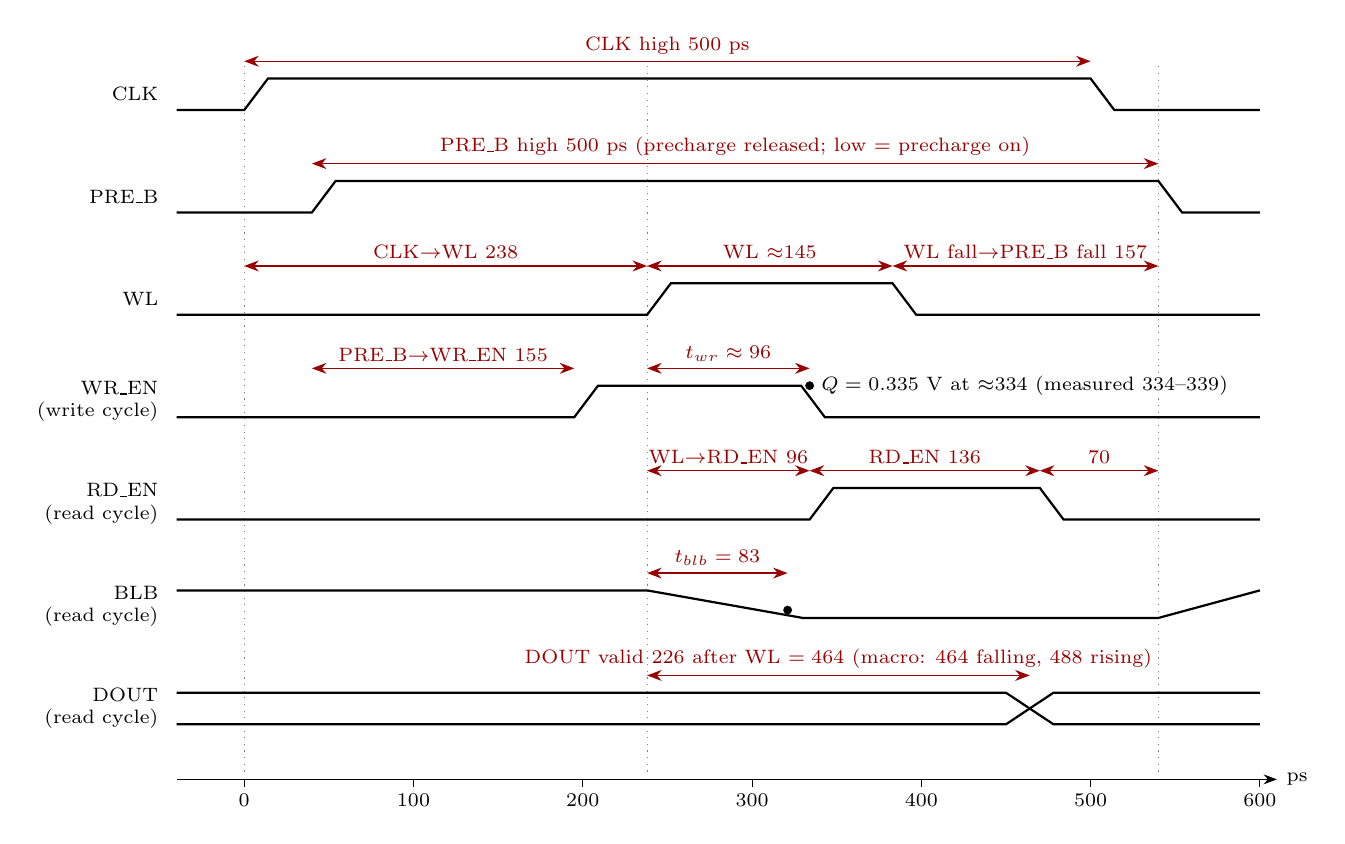
\begin{tikzpicture}[x=0.0215cm,y=1cm,font=\scriptsize,>=Stealth]
\tikzset{sig/.style={thick},dm/.style={<->,red!60!black,line width=.5pt},guide/.style={dotted,gray}}
\newcommand{\pulse}[3]{\draw[sig] (-40,#1)--(#2,#1)--({#2+14},{#1+.4})--(#3,{#1+.4})--({#3+14},#1)--(600,#1);}
\newcommand{\dm}[5]{\draw[dm] (#2,#1)--(#3,#1) node[midway,above=-1pt,#5]{#4};}
% guides
\draw[guide] (0,-.4)--(0,8.6); \draw[guide] (238,-.4)--(238,8.6); \draw[guide] (540,-.4)--(540,8.6);
% signals (low level y0, high level y0+.4)
\node[anchor=east] at (-45,8.2) {CLK}; \pulse{8}{0}{500}
\node[anchor=east] at (-45,6.9) {PRE\_B}; \pulse{6.7}{40}{540}
\node[anchor=east] at (-45,5.6) {WL}; \pulse{5.4}{238}{383}
\node[anchor=east,align=right] at (-45,4.3) {WR\_EN\\(write cycle)}; \pulse{4.1}{195}{329}
\node[anchor=east,align=right] at (-45,3.0) {RD\_EN\\(read cycle)}; \pulse{2.8}{334}{470}
\node[anchor=east,align=right] at (-45,1.7) {BLB\\(read cycle)};
\draw[sig] (-40,1.9)--(238,1.9)--(330,1.55)--(540,1.55)--(600,1.9);
\node[anchor=east,align=right] at (-45,.4) {DOUT\\(read cycle)};
\draw[sig] (-40,.6)--(450,.6)--(478,.2)--(600,.2); \draw[sig] (-40,.2)--(450,.2)--(478,.6)--(600,.6);
% dimensions
\dm{8.62}{0}{500}{CLK high 500 ps}{}
\dm{7.32}{40}{540}{PRE\_B high 500 ps (precharge released; low $=$ precharge on)}{}
\dm{6.02}{0}{238}{CLK$\to$WL 238}{}
\dm{6.02}{238}{383}{WL $\approx$145}{}
\dm{6.02}{383}{540}{WL fall$\to$PRE\_B fall 157}{}
\dm{4.72}{40}{195}{PRE\_B$\to$WR\_EN 155}{}
\dm{4.72}{238}{334}{$t_{wr}\approx96$}{}
\dm{3.42}{238}{334}{WL$\to$RD\_EN 96}{}
\dm{3.42}{334}{470}{RD\_EN 136}{}
\dm{3.42}{470}{540}{70}{}
\dm{2.12}{238}{321}{$t_{blb}=83$}{}
\dm{.82}{238}{464}{DOUT valid 226 after WL $=464$ (macro: 464 falling, 488 rising)}{}
% markers
\fill (334,4.5) circle (1.6pt) node[right=3pt,fill=white,inner sep=1pt] {$Q=0.335$ V at $\approx$334 (measured 334--339)};
\fill (321,1.65) circle (1.6pt);
% time axis
\draw[->] (-40,-.5)--(610,-.5) node[right] {ps};
\foreach \t in {0,100,...,600}{\draw (\t,-.5)--(\t,-.6) node[below=-1pt]{\t};}
\end{tikzpicture}
}
\caption{Annotated timing, $t_{clk}=1$ ns, times in ps from the rising CLK edge. Measured: CLK$\to$WL 238, WL pulse $\approx145$, WL$\to$RD\_EN 96, RD\_EN width 136, WL and RD\_EN fall 157 and 70 ps before PRE\_B, PRE\_B rises 155 ps before WR\_EN, $t_{blb}=83$, write $\approx96$ after WL, DOUT 226 after WL.}\end{figure}

%==============================================================
\section{Column circuits (2.3)}
Unit tests use $C_{BL}=3.5$ fF. Extracted and $+20\%$ extracted loads are in Table~\ref{tab:scale}.

\subsection{Precharge}
Three PMOS, 2 fins each: one per bitline to VDD and one equalizer, gated by PRE\_B. PRE\_B follows CLK, so precharge is on while CLK is low and off while CLK is high. At $T_{CLK,\min}=0.69$ ns the low phase is $345$ ps, which is the recovery window. The 2-fin \code{p1svt} is taken at $I_{\rm on,p}=12$ $\mu$A ($\approx0.5\times$ the $25$ $\mu$A n-pass of the cell). Restore of $\Delta V=V_{DD}-V_M$ is
\begin{equation}
t_{\rm pre}=\frac{C_{BL}(V_{DD}-V_M)}{I_{\rm on,p}}.
\end{equation}
That is $124$ ps at $3.5$ fF, $304$ ps at $8.59$ fF, and $364$ ps at $10.3$ fF. The $3.5$ fF and extracted cases finish inside the $345$ ps low. At $+20\%$ of extracted, $t_{\rm pre}$ overruns the half-period by $19$ ps; recovery is a $40$ ps stretch of $T_{CLK}$ ($0.73$ ns) or a $45\%$ duty so the low phase is $380$ ps. In every passing column test the bitlines are already at VDD when WL rises.

\begin{figure}[H]\centering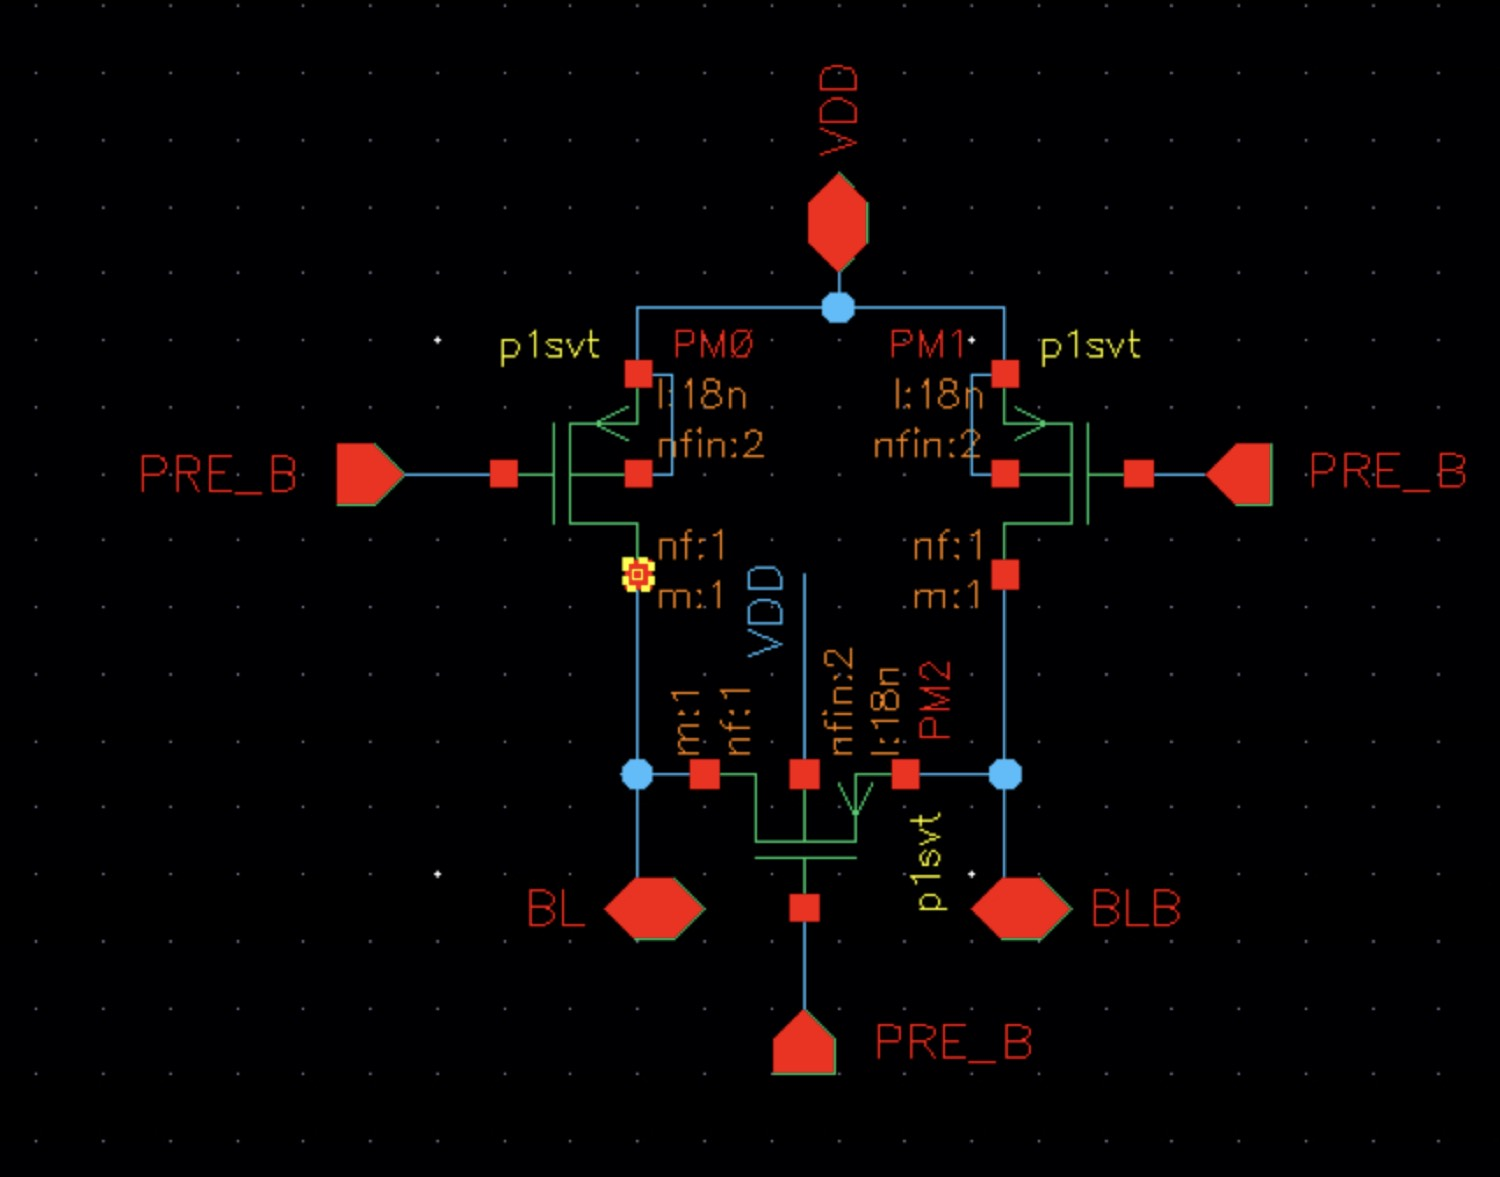
\includegraphics[width=.38\linewidth]{precharge_schematic}
\caption{\code{precharge}: three 2-fin PMOS, gate PRE\_B.}\end{figure}

\subsection{Write driver}
Four NMOS pull-downs plus a 2+2-fin inverter. A small driver loses the race against the undriven bitline: the cell discharges BLB through its pass-gate, pins $\overline Q$ low and blocks its own feedback.
\begin{table}[H]\centering\small\caption{Driver sizing ($V_{DD}=0.8$ V, $C_{BL}=3.5$ fF, $pw\_w1=0.3$ ns).}\label{tab:drv}
\begin{tabular}{@{}rlrrr@{}}\toprule nfin & Write 0 & $t_{wr0}$ (ps) & $t_{wr1}$ (ps) & Lowest BLB (mV)\\\midrule
2 & fail, Q stalls at 0.66 V & -- & -- & $\sim$0\\
4 & fail, Q stalls at 0.38 V & -- & -- & $\sim$60\\
5 & pass & 153 & 154 & $\sim$190\\
6 & pass & 121 & 121 & $\sim$260\\
\textbf{8} & pass & 96 & 96 & $\sim$345\\\bottomrule\end{tabular}
\end{table}
\begin{center}\small\begin{tabular}{rll}\toprule WL at 50\% & $C_{BL}=3.5$ fF & $4.2$ fF ($+20\%$ of $3.5$ fF)\\\midrule
$\sim$60, 80, 100 ps & fail & fail\\
$\sim$120, 140, 170 ps & pass, 96 ps & pass, 102 ps\\\bottomrule\end{tabular}\end{center}
nfin 5 is the smallest that writes. nfin 8 writes in $96$ ps ($102$ ps at $+20\%$ of $3.5$ fF) and is the design point: $0.77$ $\mu$m$^2$ over nfin 6 (3\% of the array) buys $25$ ps, and $T_{CLK,\min}$ is set by the read, not by this $6$ ps. The $3.5\to4.2$ fF slope is $8.6$ ps/fF, so the extracted $8.59$ fF writes in $140$ ps and $+20\%$ extracted ($10.3$ fF) in $154$ ps. Minimum write pulse $100$--$120$ ps at 50\% at the test loads; $160$ ps at $10.3$ fF.
\begin{figure}[H]\centering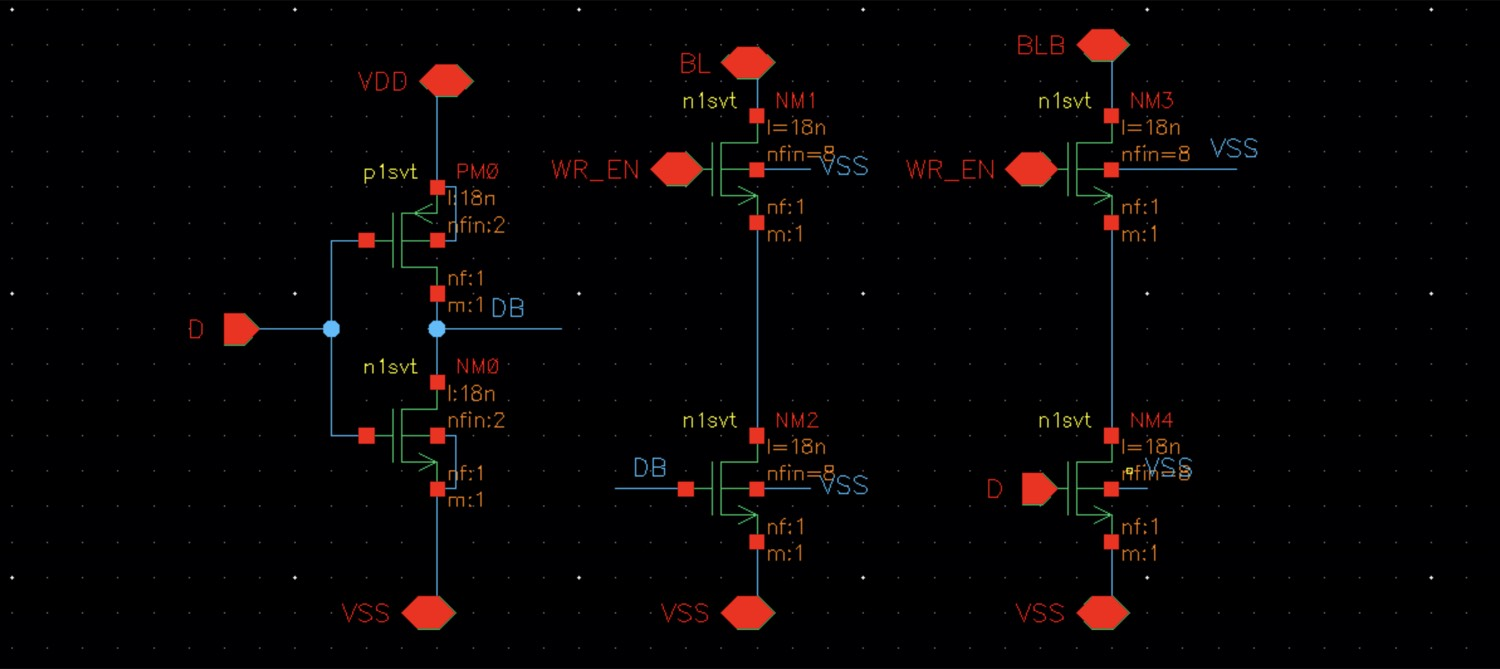
\includegraphics[width=.48\linewidth]{write_driver_schematic_nfin8}\hfill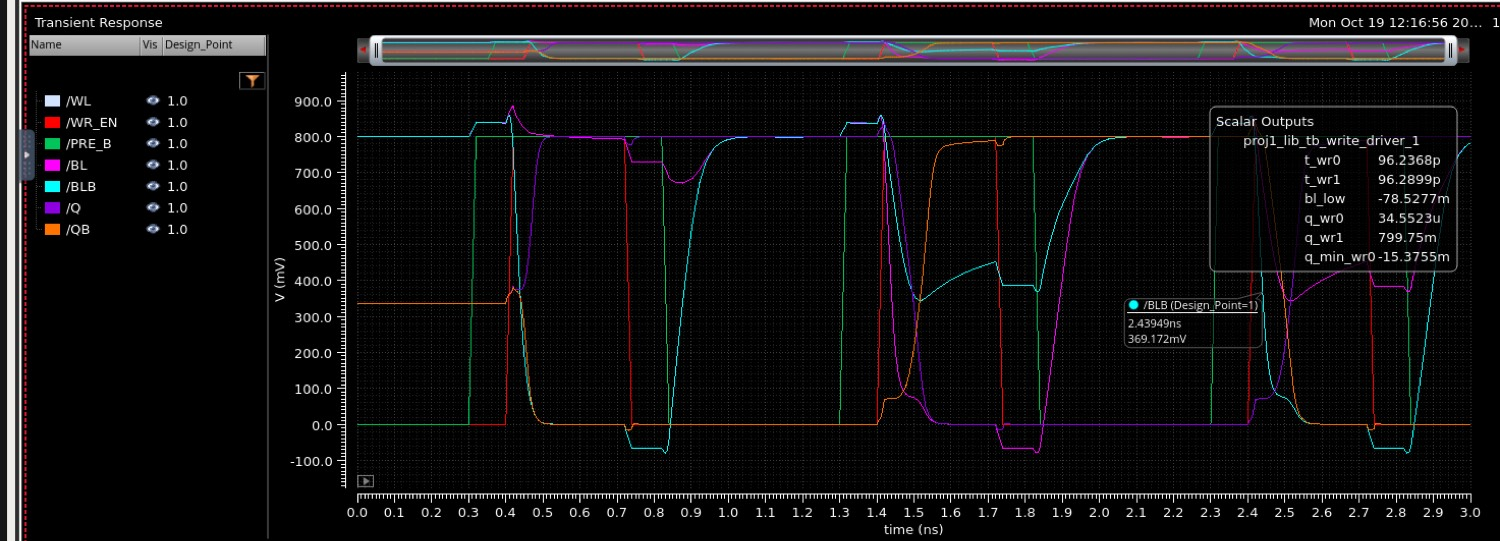
\includegraphics[width=.48\linewidth]{write_driver_tran_nfin8}
\caption{Write driver at nfin 8, and write-0 / write-1 ($q_{wr0}=35$ $\mu$V, $q_{wr1}=799.8$ mV, $t_{wr0}=96$ ps).}\end{figure}

\subsection{Read path}
Full-swing inverter on BLB, no sense amplifier. Chosen 2:2 (PMOS 2, NMOS 2), $V_M=376$ mV, so BLB must fall $0.424$ V to flip RD. The $140$ ps WL pulse gives $57$ ps of slack over the $83$ ps bitline time at $3.5$ fF. A 4:2 inverter would switch at $0.415$ V, save $\approx7$ ps and add 8 fins ($0.19$ $\mu$m$^2$); it is off the critical path because the write sets the pulse.
\begin{figure}[H]\centering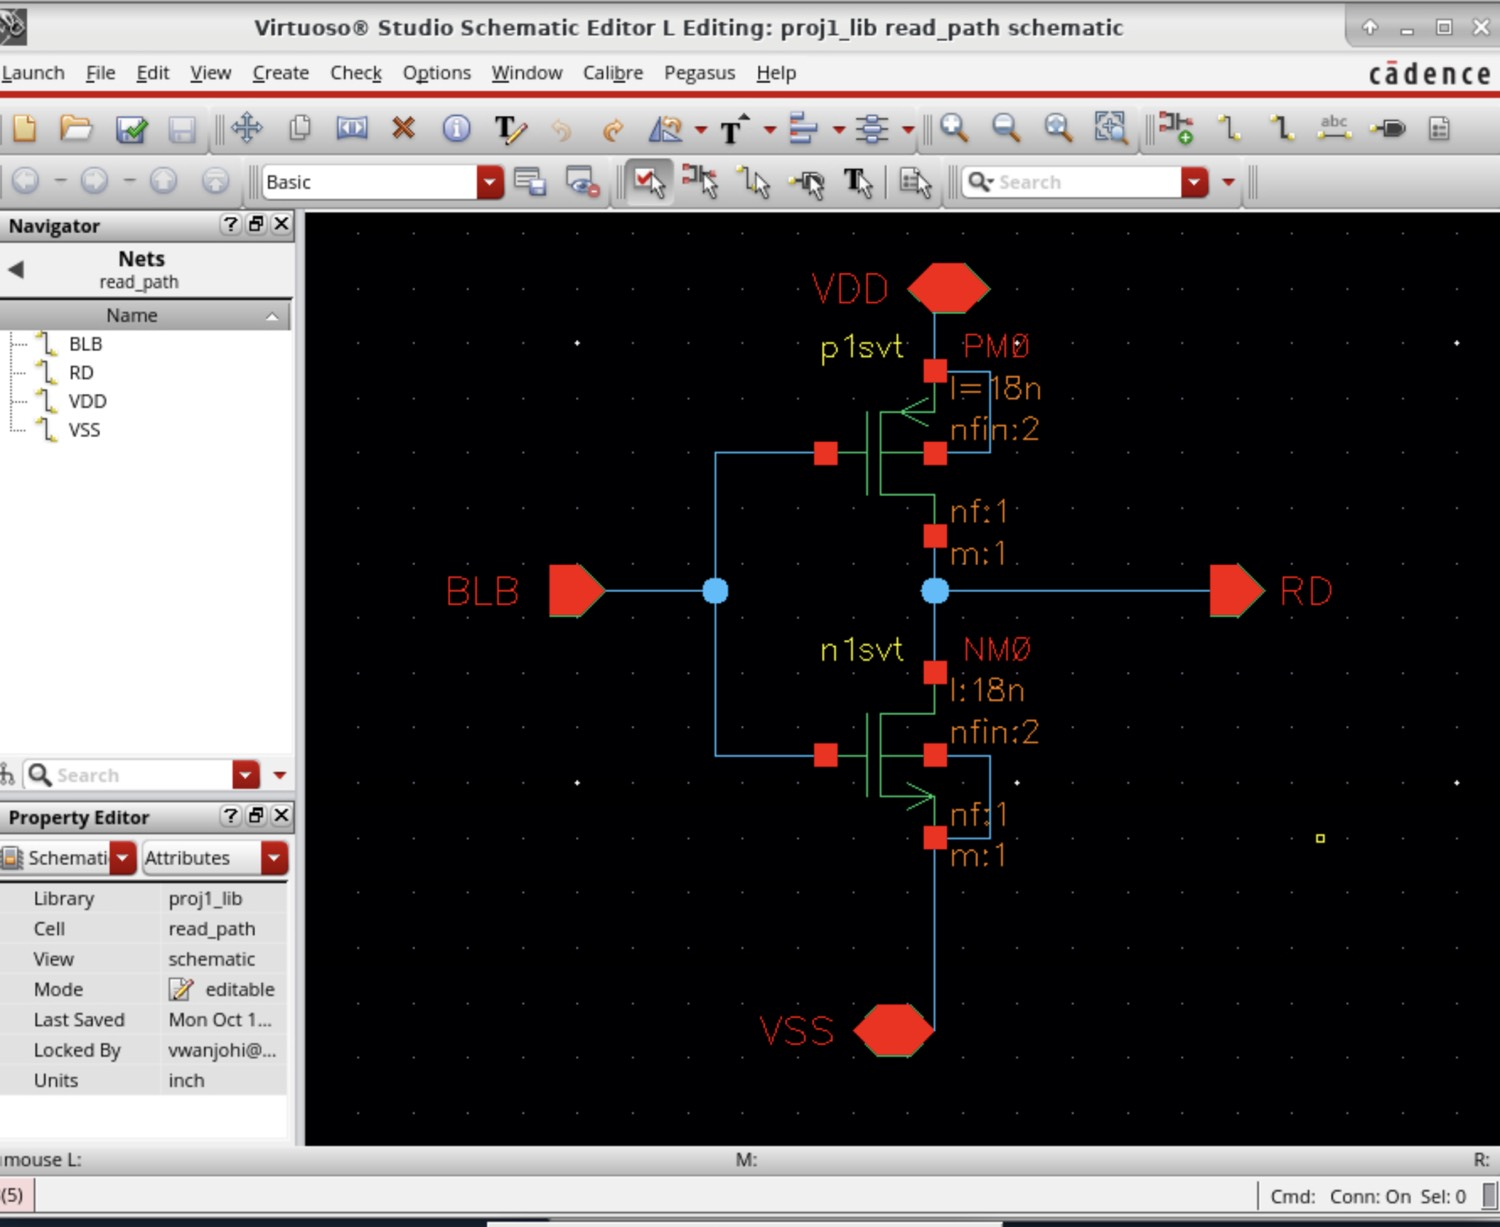
\includegraphics[width=.4\linewidth]{read_path_schematic_library_view_2to2}\hfill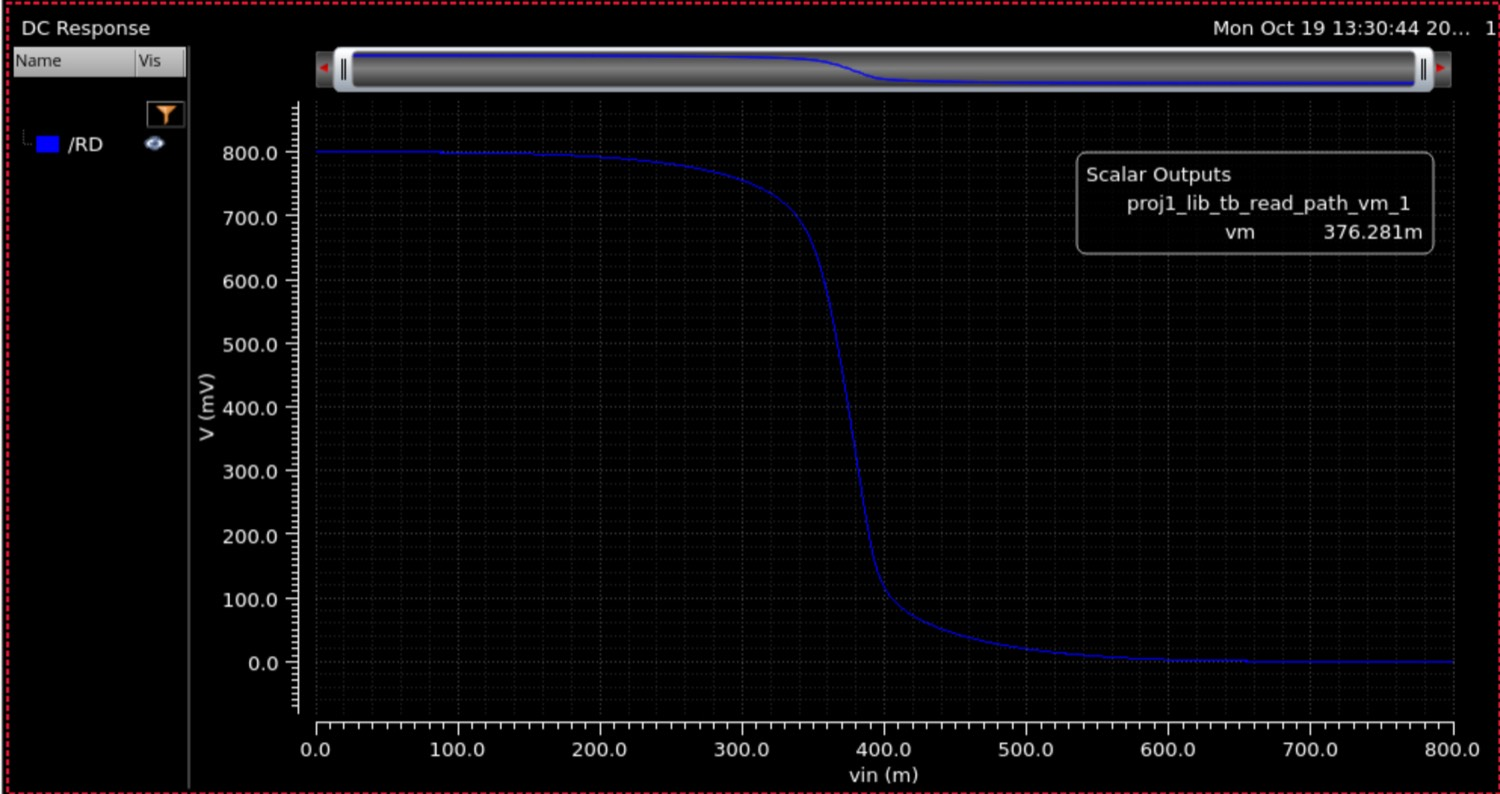
\includegraphics[width=.52\linewidth]{read_path_vtc_2to2}
\caption{\code{read\_path} (2:2) and its transfer curve, $V_M=376$ mV.}\end{figure}

\subsection{Output latch}
All devices 2 fins. Enable-pulse sweep, $c_{dout}=1$ fF; hold-1 $>0.72$ V, hold-0 $<0.08$ V. $10$ ps fails (never captures a 1). $20$ ps and wider pass. Design width $120$ ps (column test).
\begin{figure}[H]\centering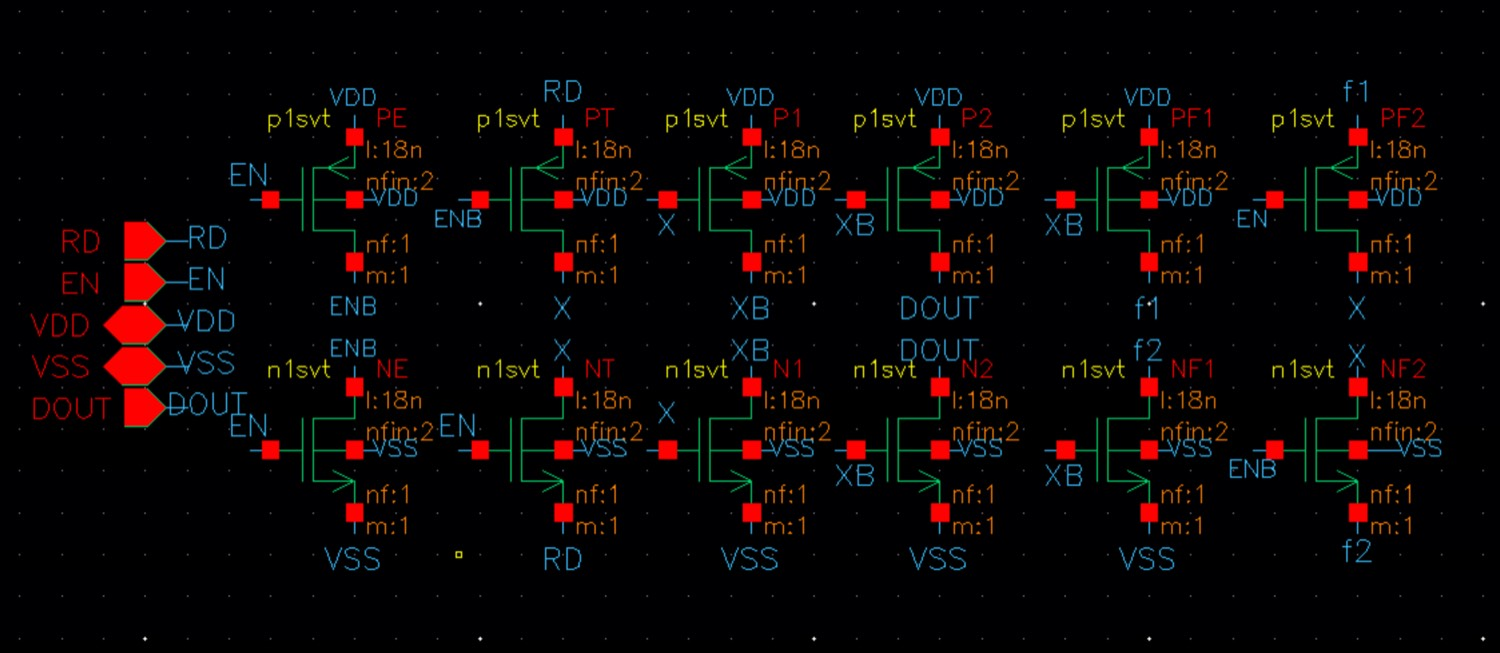
\includegraphics[width=.34\linewidth]{out_latch_schematic}\hfill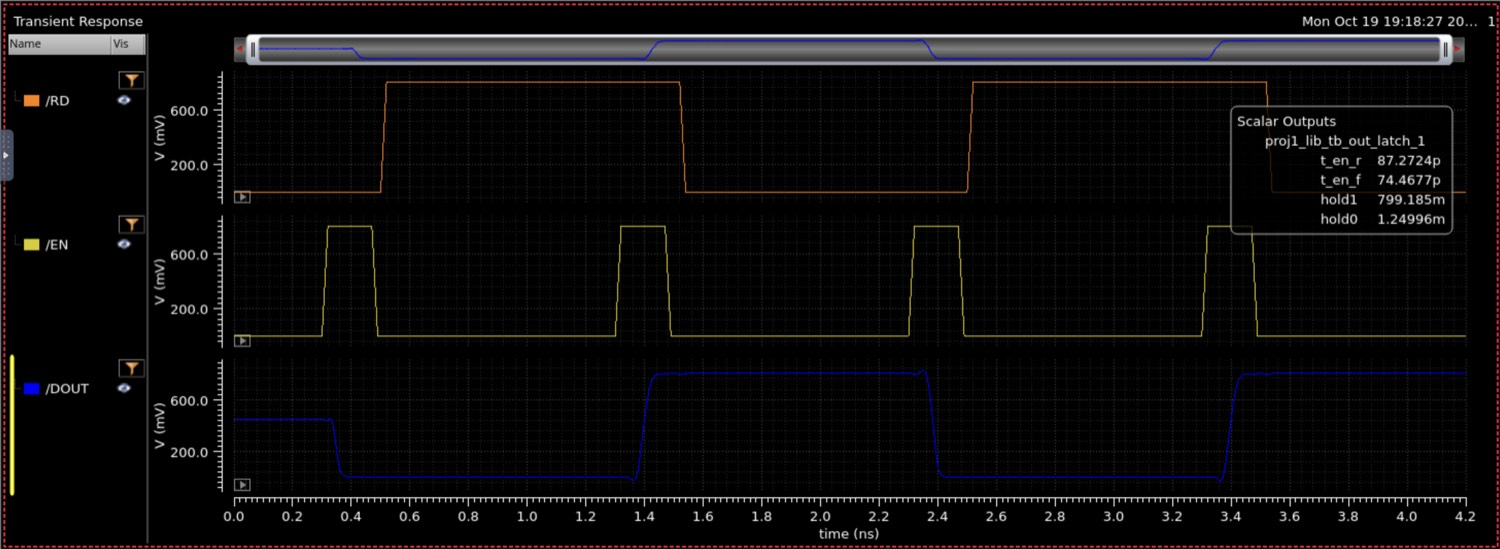
\includegraphics[width=.62\linewidth]{out_latch_tran_en_delay300p}
\caption{\code{out\_latch} and unit test at $150$ ps: DOUT writes only while EN is high.}\end{figure}

\subsection{Read column}
Cell, write driver, precharge, read path and latch together: write 1, read, write 0, read, write 1, read. Sweep of latch delay \code{rd\_dly} and width \code{pw\_rden} (24 points). All checks pass except the third read at \code{pw\_rden}$=40$ p.
\begin{center}\small\begin{tabular}{rrrrrr}\toprule \code{rd\_dly} & 40p & 80p & 120p & 160p & $t_{acc0}$\\\midrule
1.48n & fail & 247 & \textbf{226} & 226 & 165\\
1.52n & fail & 235 & 235 & 235 & 205\\
1.56n--1.68n & fail & $+40$ ps per $40$ ps of delay & & & $+40$ ps\\\bottomrule\end{tabular}\end{center}
\textbf{Chosen: \code{rd\_dly}$=1.48$ n, \code{pw\_rden}$=120$ p.} BLB hits $0.376$ V $83$ ps after WL; DOUT valid $165$ ps (read 0) and $226$ ps (read 1). Cell undisturbed: $q_{rd1}=799.7$ mV, $q_{rd0}=39$ $\mu$V.
\begin{figure}[H]\centering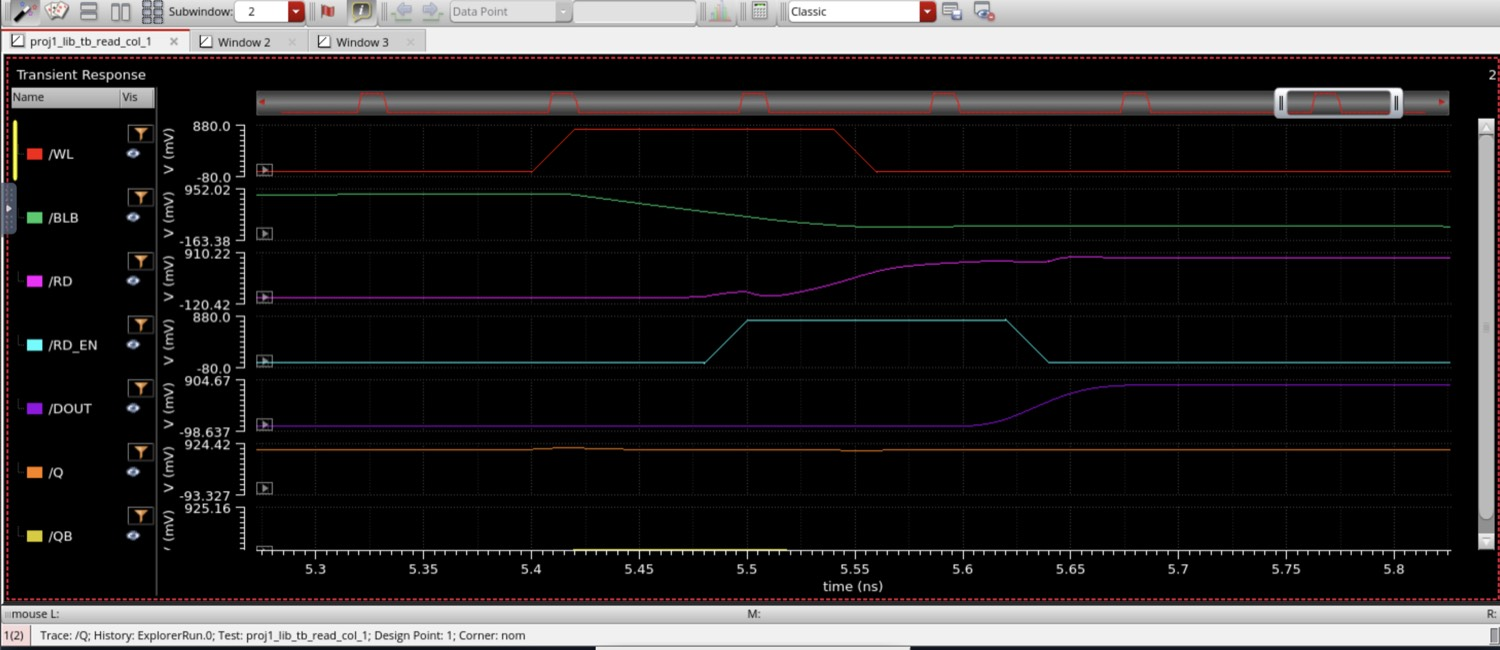
\includegraphics[width=.92\linewidth]{read_col_tran_1p48n_120p_zoom_read3_stacked_BEST}
\caption{Cycle-6 read of a 1, $C_{BL}=3.5$ fF: BLB crosses $0.376$ V at $83$ ps; DOUT valid $226$ ps after WL.}\end{figure}

%==============================================================
\section{Controller (2.4)}\label{sec:ctrl}
Inputs CLK, WE, ADDR, DIN. Outputs A, AB, D, PRE\_B, WL\_EN, WR\_EN, RD\_EN. Input latches (\code{out\_latch}, enable CLKBL from its own \code{inv\_2x}) hold ADDR, DIN and WE while CLK is high. PRE\_B $=\code{inv\_2x}$(CLKB) follows CLK; the precharge PMOS conduct when PRE\_B is low, so precharge is on while CLK is low. WL\_EN $=$ CLKBUF AND (CLKBUF through 7 \code{inv\_u}): a one-shot on each rising edge. WR\_EN $=$ WL\_EN AND WE. RD\_EN $=$ (WL\_EN through 8 \code{inv\_u}) AND $\overline{\rm WE}$.
\begin{figure}[H]\centering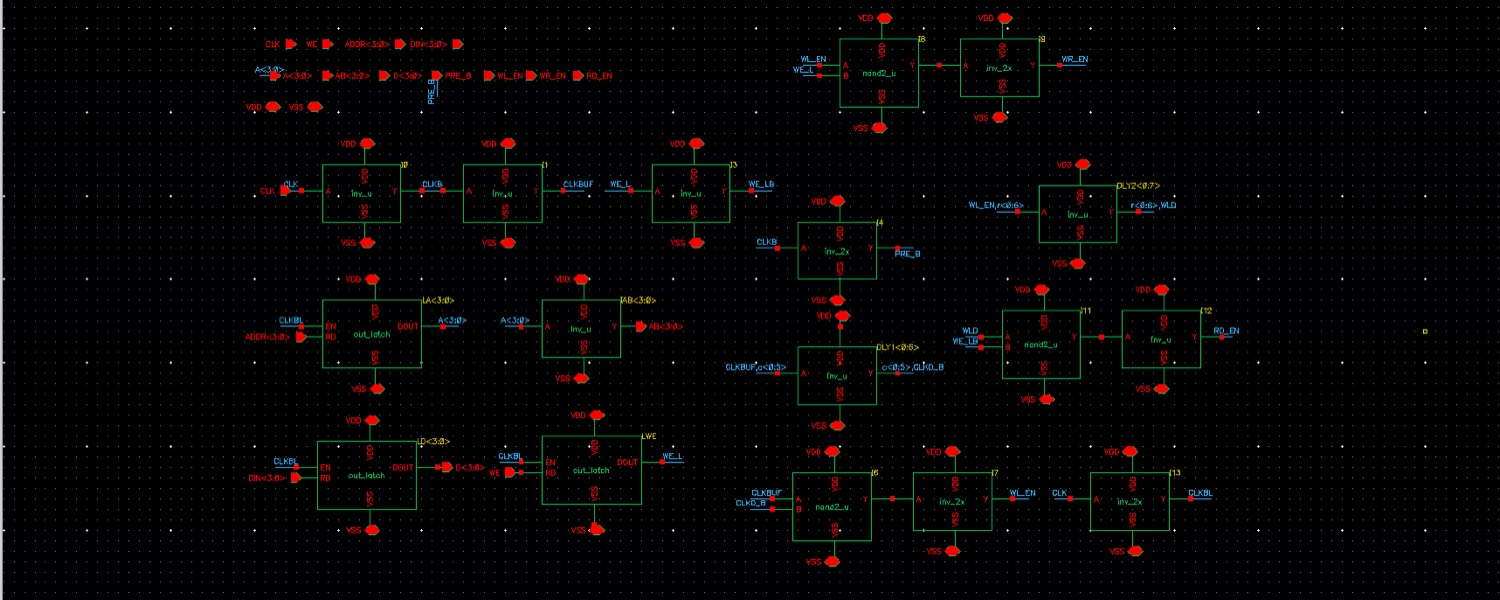
\includegraphics[width=.88\linewidth]{controller_schematic}
\caption{\code{controller}: input latches, WL\_EN one-shot (DLY1), WR\_EN and RD\_EN (DLY2).}\end{figure}

\begin{table}[H]\centering\small\caption{Controller timing at $0.4$ V crossings, before and after moving the latch enable onto its own inverter.}
\begin{tabular}{@{}lrrl@{}}\toprule Output & Before & After & \\\midrule
CLK $\to$ WL & 356 ps & \textbf{238 ps} & \\
RD\_EN fall before PRE\_B fall & 30 ps & \textbf{70 ps} & thinnest margin\\
WL fall before PRE\_B fall & 118 ps & 157 ps & \\
PRE\_B rise before WR\_EN rise & 178 ps & 155 ps & \\
WL $\to$ RD\_EN & 96 ps & 96 ps & column needs $\ge80$\\
RD\_EN width & 136 ps & 136 ps & column needs $\ge100$\\
WL\_EN width & 134 ps & 134 ps & write needs $120$--$140$\\\bottomrule\end{tabular}
\end{table}
No spurious pulses: RD\_EN peaks at $3.3$ mV in a write cycle, WR\_EN at $0.41$ mV in a read cycle. Margins after the CLKBL change: WL\_EN width $+14$ ps over $120$ ps; RD\_EN lead $+16$ ps over $80$ ps; RD\_EN width $+36$ ps over $100$ ps; RD\_EN before precharge $+70$ ps; WL before precharge $+157$ ps; PRE\_B before WR\_EN $+155$ ps.
\begin{figure}[H]\centering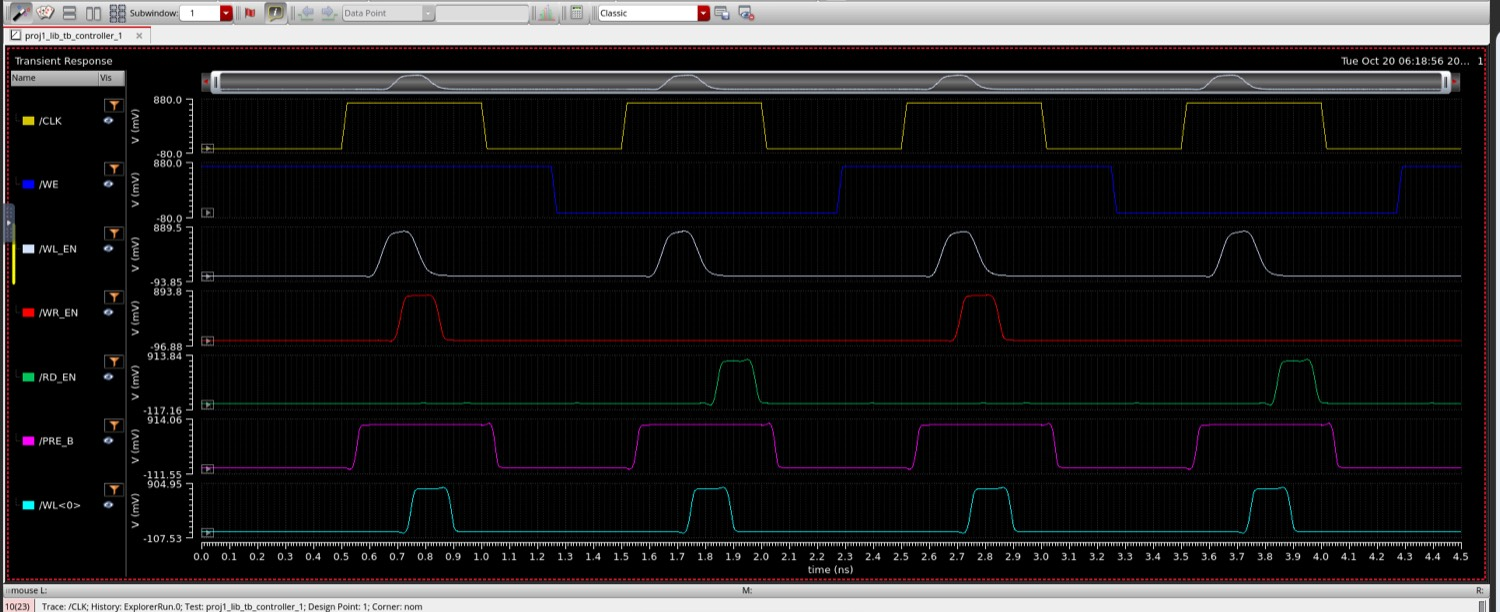
\includegraphics[width=.88\linewidth]{tb_controller_tran}
\caption{Controller transient: WR\_EN in write cycles only, RD\_EN in read cycles only; WL ends before PRE\_B falls.}\end{figure}

\textbf{$+20\%$ of extracted $C_{BL}$.} Extracted $C_{BL}=8.59$ fF; $+20\%$ is $10.3$ fF. From Table~\ref{tab:scale}: write $154$ ps, $t_{blb}$ $245$ ps, $t_{\rm pre}$ $364$ ps. The $140$ ps WL pulse and the $345$ ps CLK-low window are both short of those three numbers. Recovery, without resizing the cell:
\begin{itemize}\setlength{\itemsep}{1pt}
\item DLY1: two extra \code{inv\_u} ($\approx20$ ps) on WL\_EN, then two more if the scaled $t_{blb}$ is the bound, for a $\approx180$ ps pulse.
\item DLY2: drop two inverters ($\approx20$ ps) so RD\_EN still opens after the bitline crosses $V_M$.
\item Clock: stretch $T_{CLK}$ to $0.73$ ns, or keep a $45\%$ duty so CLK-low is $380$ ps, covering the $364$ ps restore.
\end{itemize}
At the column-test $+20\%$ ($4.2$ fF) none of this is needed: write $+6$ ps, $t_{blb}$ $83\to100$ ps, both inside $140$ ps. The $70$ ps RD\_EN-to-precharge margin is the one that shrinks if the read stretches. The $70$ ps margin does not set $T_{CLK,\min}$: it would have vanished near $0.86$ ns if the half-period shrank around a fixed pulse, yet the macro passes to $0.69$ ns.

%==============================================================
\section{Verification (2.5)}
\code{tb\_sram\_macro}: CLK, WE and ADDR through two \code{inv\_u} each; $1$ fF on DOUT. Address is a binary counter, one step per cycle. WE high for 16 cycles (write all words), low for 16 (read all), repeating. DIN $=\{X,\bar X,X,\bar X\}$ with $X=a_0\oplus ph$, so each word is 0101 or 1010 alternating by row; $ph$ flips at $32.25\,t_{clk}$ and complements every word. \code{err1}/\code{err2} are the peak DOUT error in the checkerboard and complement read windows against $0.1$ V; \code{err3} is test (iii).
\begin{figure}[H]\centering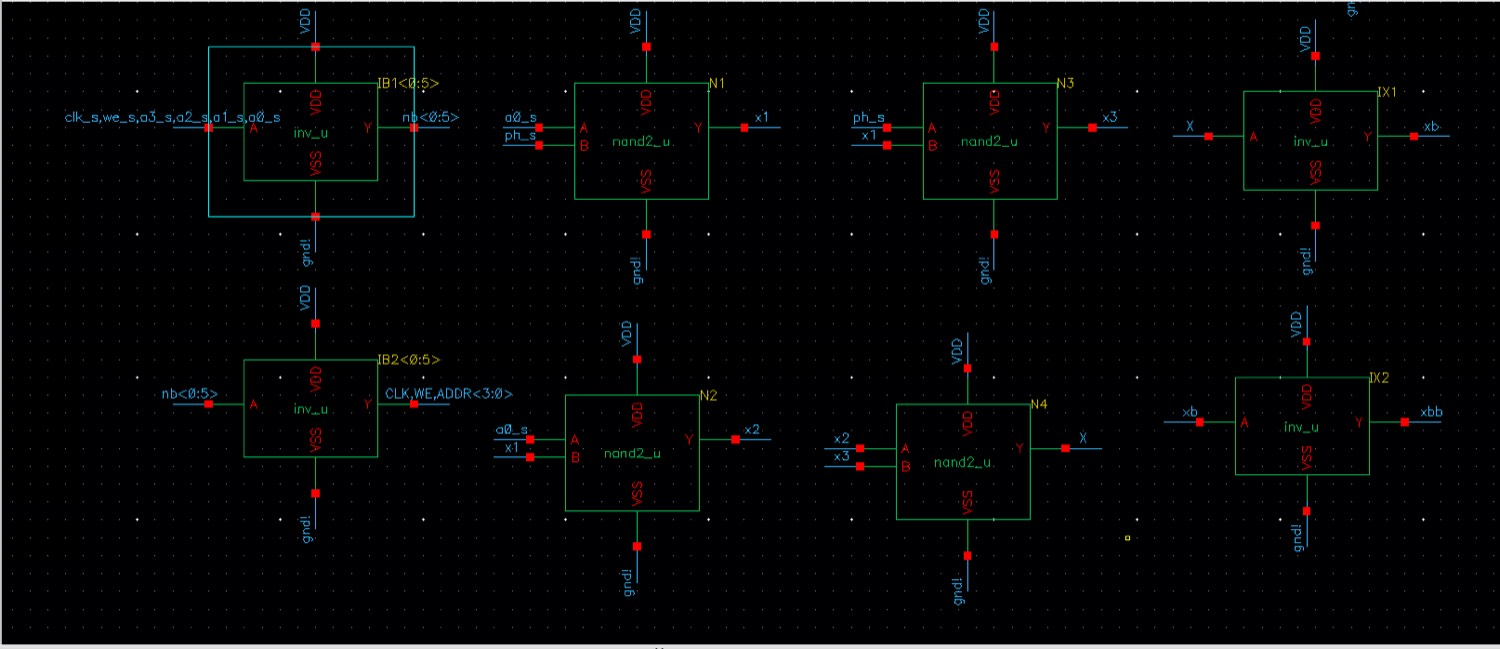
\includegraphics[width=.85\linewidth]{tb_sram_macro_buffers_and_data_gates}
\caption{Input buffers and the NAND XOR that builds DIN.}\end{figure}

\begin{table}[H]\centering\small\caption{Pass/fail at $t_{clk}=1$ ns.}\label{tab:pass}
\begin{tabularx}{\linewidth}{@{}p{.46\linewidth}Xl@{}}\toprule Test & Error & \\\midrule
(i) checkerboard write, read all 16 & \code{err1} $=174$ $\mu$V & \textbf{pass}\\
(ii) complement overwrite, read all 16 & \code{err2} $=174$ $\mu$V & \textbf{pass}\\
(iii) row 15, read immediately after a write of the opposite value & \code{err3} $=174$ $\mu$V & \textbf{pass}\\\bottomrule\end{tabularx}
\end{table}
\begin{figure}[H]\centering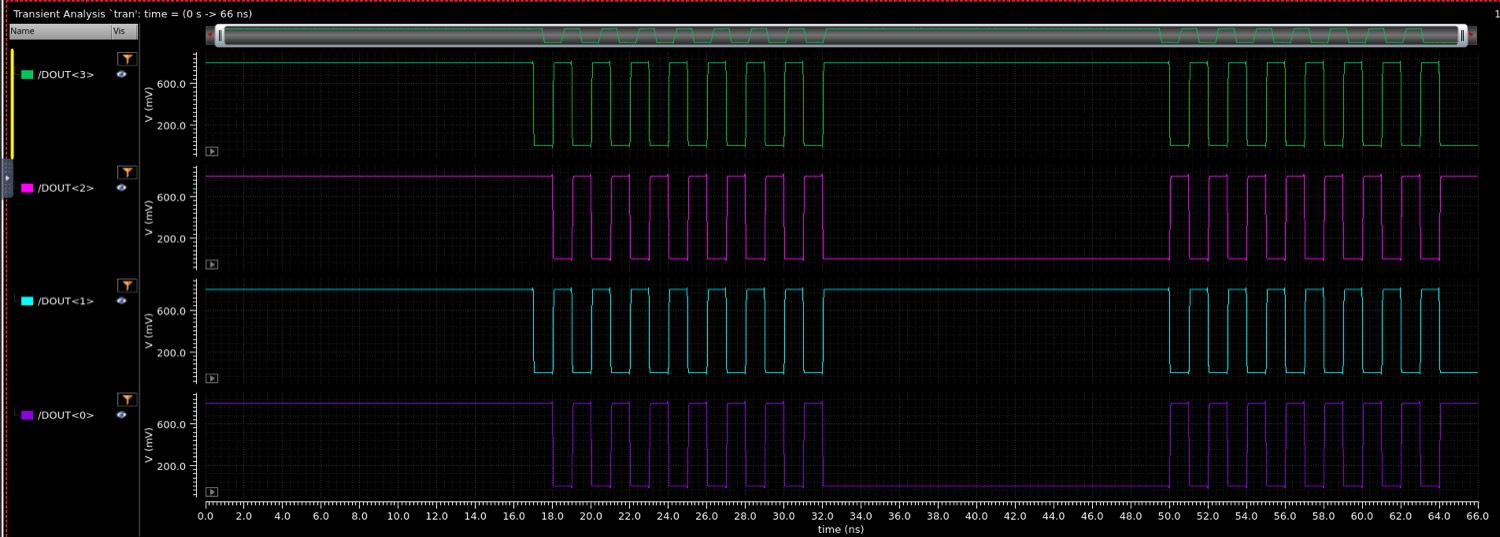
\includegraphics[width=.85\linewidth]{tb_sram_macro_tran_dout}
\caption{DOUT$\langle3{:}0\rangle$: bits 3,1 opposite bits 2,0. DOUT holds while WE is high.}\end{figure}
\begin{figure}[H]\centering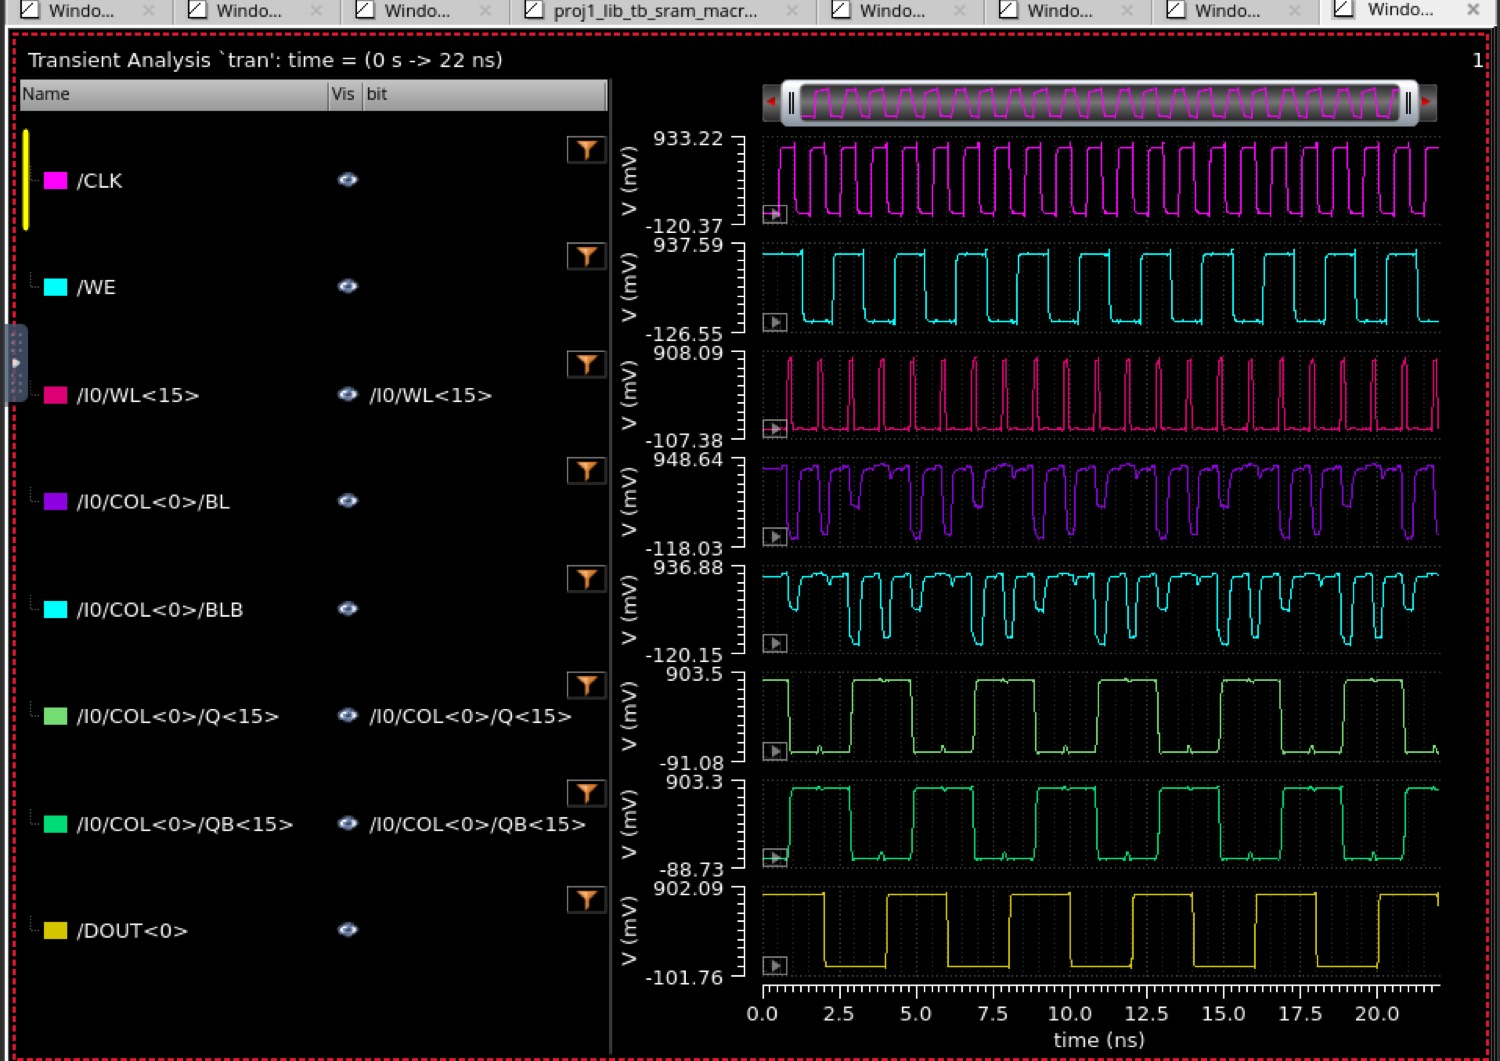
\includegraphics[width=.56\linewidth]{tb_sram_macro_row15_all_signals_22ns_BEST}\hfill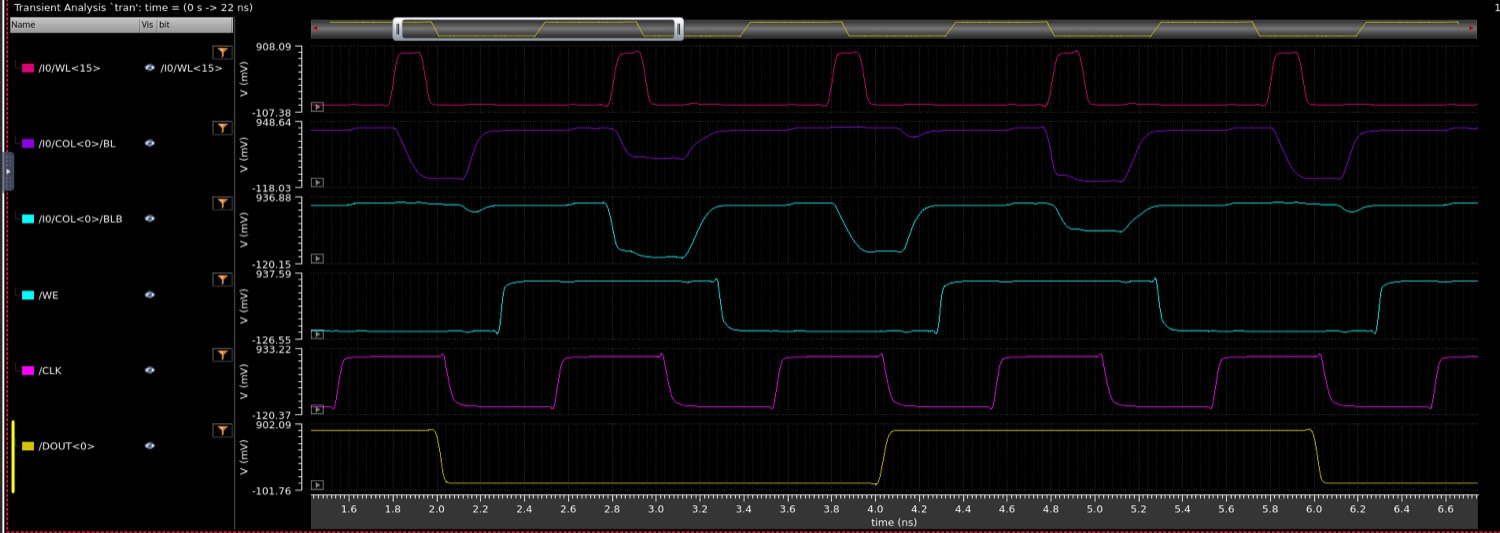
\includegraphics[width=.42\linewidth]{tb_sram_macro_row15_wl_bl_we_clk_dout_zoom_BEST}
\caption{Test (iii), row 15. WE alternates every cycle; each read returns the value just written. DOUT changes $\approx0.5$ ns after the read edge.}\end{figure}

\textbf{Write time} (later of $Q$ and $\overline Q$ crossing $0.335$ V, from the CLK edge, row 15): $339$ ps (write 1), $334$ ps (write 0). That is the controller's $238$ ps to WL plus the column's $96$ ps. \textbf{Read access} (CLK to DOUT$\langle1\rangle$, $0.4$ V): $464$ ps falling, $484$ ps rising at $1$ ns; $488$ ps rising at $T_{CLK,\min}$.
\begin{figure}[H]\centering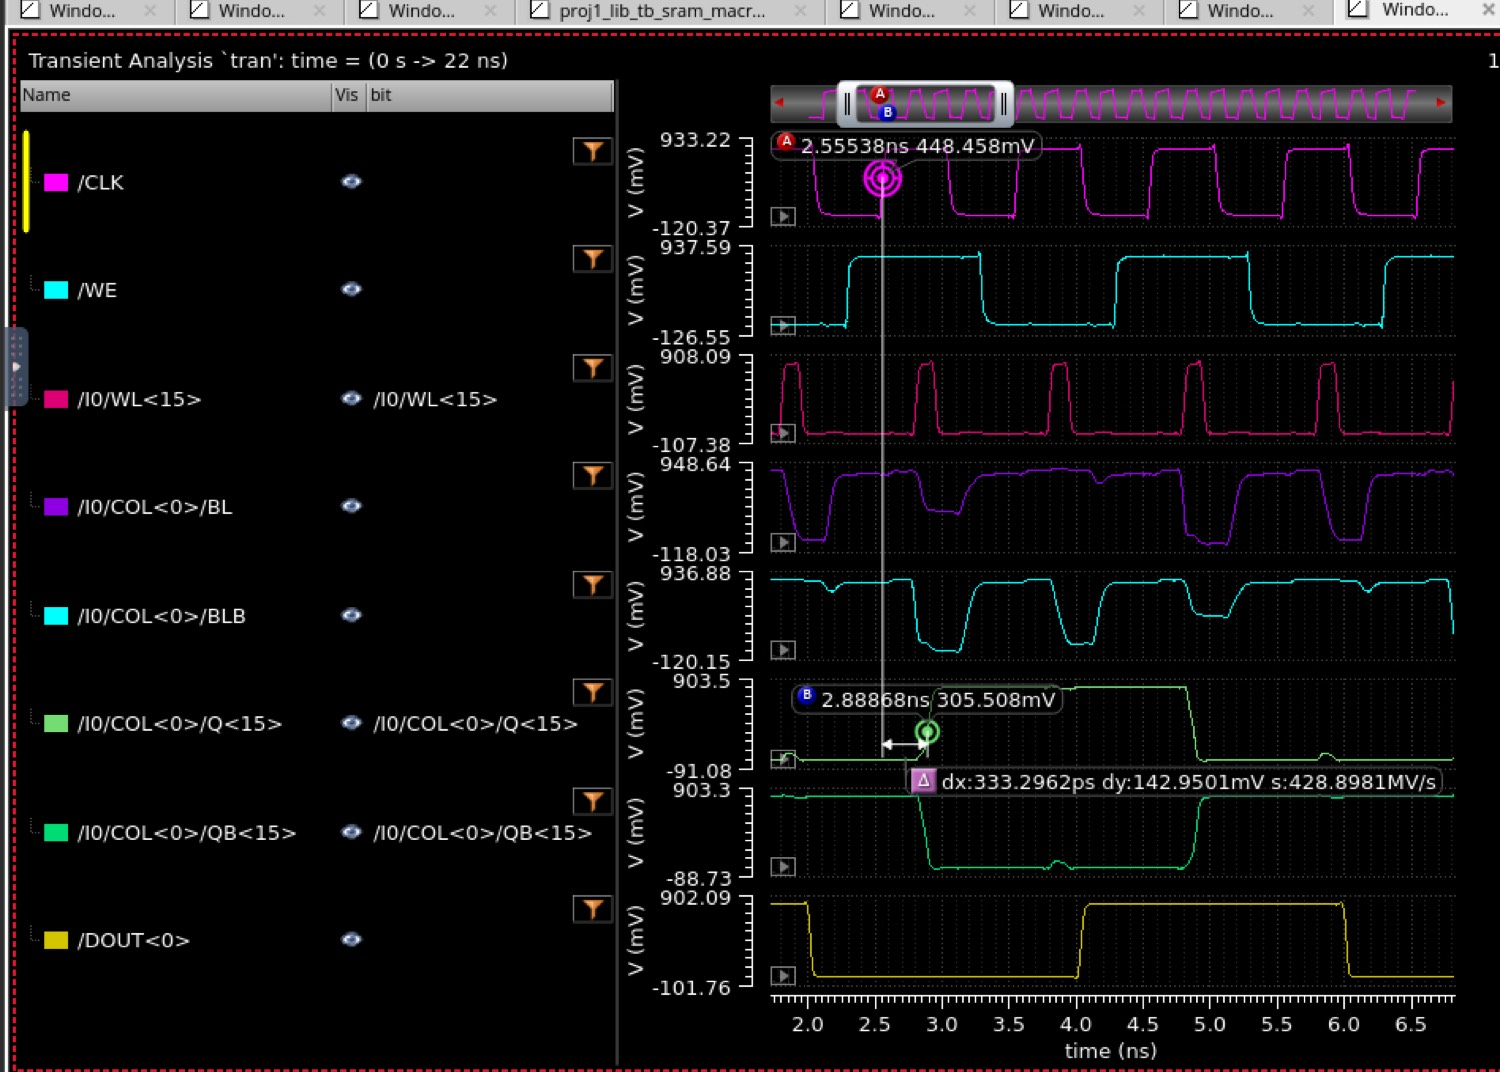
\includegraphics[width=.62\linewidth]{tb_sram_macro_write_time_markers}
\caption{Write time on row 15: CLK edge to $Q\langle15\rangle$, $333$ ps on the cursors ($339$ ps at the $0.335$ V crossing).}\end{figure}

\begin{table}[H]\centering\small\caption{Clock-period sweep. Power is the macro VDD-pin current $\times0.8$ V.}\label{tab:tclk}
\begin{tabular}{@{}rrrlrrrr@{}}\toprule $t_{clk}$ & \code{err1} & \code{err2} & & $t_{acc,f}$ & $t_{acc,r}$ & write & read\\\midrule
$1$ ns -- $750$ ps & $174$ $\mu$V -- $0.50$ mV & same & pass & 464 & 484--486 & -- & --\\
700 ps & 5.10 mV & 5.12 mV & pass & 464 & 486 & 123 $\mu$W & 113 $\mu$W\\
\textbf{690 ps} & 23.3 mV & 22.4 mV & \textbf{pass} & 464 & \textbf{488} & 124 $\mu$W & 115 $\mu$W\\
680 ps & 452 mV & 441 mV & fail & 464 & 497 & 126 $\mu$W & 118 $\mu$W\\
$\le670$ ps & 1.28 V & 1.28 V & fail & 464 & -- & 128--143 $\mu$W & 115--123 $\mu$W\\\bottomrule\end{tabular}
\end{table}
\code{err3} tracks the same cliff: $\approx30$ mV at $690$ ps, $\approx0.6$ V at $680$ ps, $1.28$ V below that. Write times stay at $339/334$ ps. $T_{CLK,\min}=0.69$ ns (10 ps resolution).
\begin{figure}[H]\centering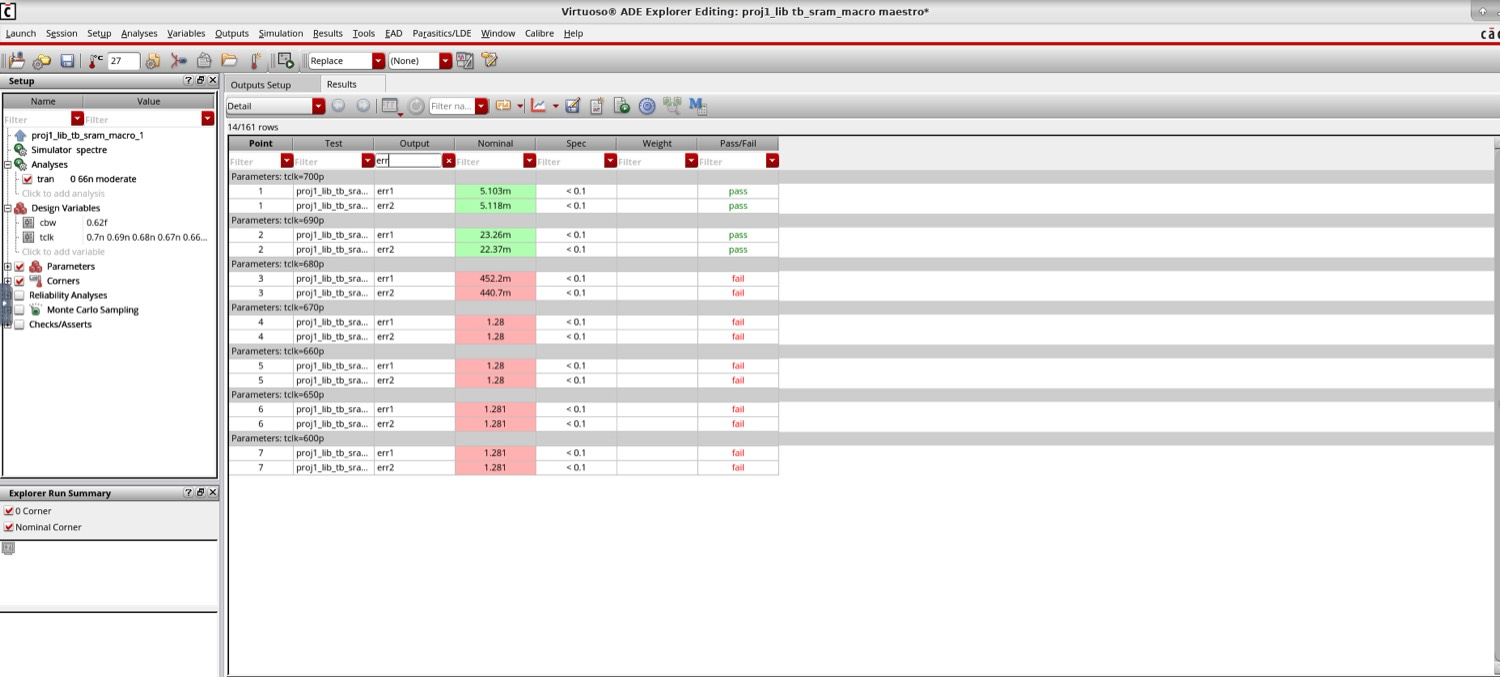
\includegraphics[width=.48\linewidth]{tb_sram_macro_tclk_600_700_err1_err2}\hfill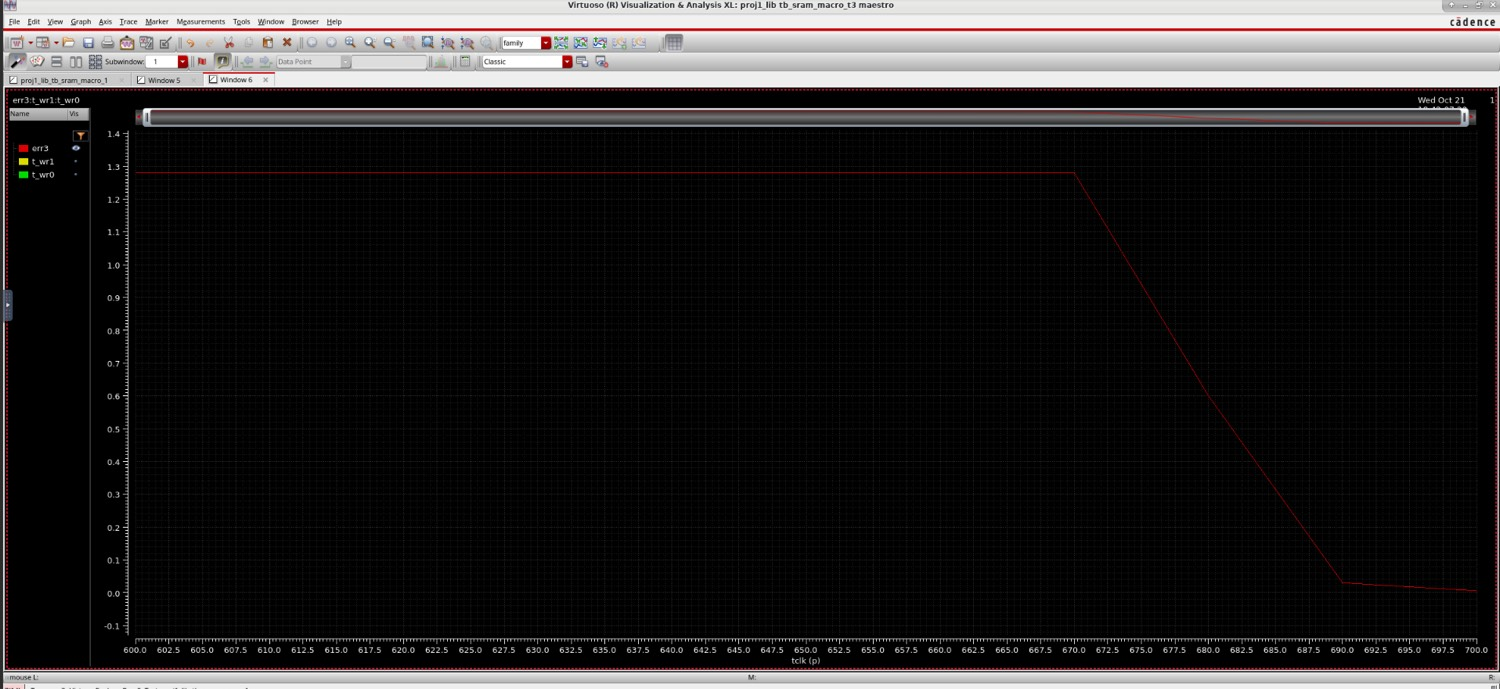
\includegraphics[width=.48\linewidth]{tb_sram_macro_tclk_sweep_err3_600_700ps}
\caption{Error versus clock period: checkerboard/complement (left) and worst-row (right). Fail below $0.69$ ns.}\end{figure}

%==============================================================
\section{Metrics and figure of merit}
$V_{DD}=0.8$ V, nominal, $27^\circ$C, $D=28$. Write power is the macro VDD-pin current $\times0.8$ V with WE high every cycle and all four columns writing (the checkerboard pass at $T_{CLK,\min}$). That is the same four-column write current as an all-0 then all-1 sweep: every cycle the write drivers fight the precharged bitlines. Standby with the clock running still fires WL\_EN on every edge (no chip-select); true standby is the clock stopped.
\begin{table}[H]\centering
\caption{Macro metrics at $T_{CLK,\min}$.}\label{tab:fom}
\begin{tabularx}{\linewidth}{@{}p{.50\linewidth}X@{}}\toprule Metric & Value\\\midrule
$T_{CLK,\min}$ & $\mathbf{0.69}$ ns (690 ps passes (i)--(iii); 680 ps fails)\\
Worst-case read access, CLK$\to$DOUT & 488 ps (DOUT$\langle1\rangle$ rising at 690 ps)\\
Worst-case write time, CLK$\to Q/\overline Q$ past $0.335$ V & 339 ps (row 15)\\
Array write power at $T_{CLK,\min}$ & 124 $\mu$W (WE high, four columns writing)\\
Checkerboard read power & 115 $\mu$W\\
Standby, CLK running (WL\_EN still fires) & 112 $\mu$W\\
Standby, CLK stopped & $3.99$ $\mu$W\\
Area: array $2.88\times8.64$ $\mu$m $+$ periphery & $24.9+29.7=\mathbf{54.6}$ $\mu$m$^2$\\
FOM $=\mathrm{Area}\cdot P_{\rm write}\cdot T_{CLK,\min}$ & $54.6\times124\times0.69\approx\mathbf{4.7\times10^3}$ $\mu$m$^2\cdot\mu$W$\cdot$ns\\\bottomrule\end{tabularx}
\end{table}
\begin{figure}[H]\centering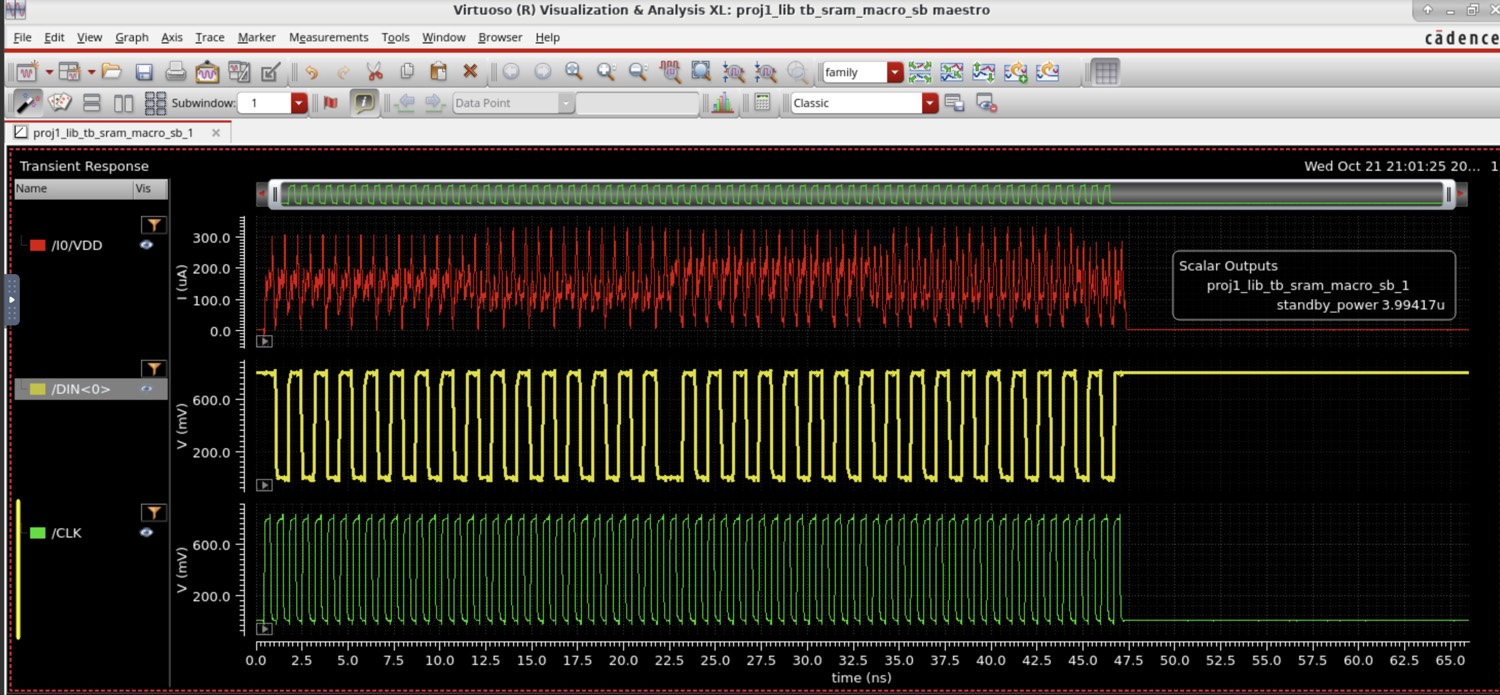
\includegraphics[width=.62\linewidth]{tb_sram_macro_sb_tran}
\caption{Standby: after the clock stops ($\approx47$ ns) the VDD current falls to leakage, $3.99$ $\mu$W.}\end{figure}

\section*{Trade-offs}
\begin{itemize}\setlength{\itemsep}{2pt}
\item \textbf{Write driver.} nfin 5 is the smallest that writes ($153$ ps). nfin 8 is $96$ ps for $0.77$ $\mu$m$^2$ over nfin 6. Kept, because $T_{CLK}$ is set by the read.
\item \textbf{Read inverter 2:2.} Saves 8 fins versus 4:2 and costs $\approx7$ ps, off the critical path.
\item \textbf{2-2 predecode versus flat NAND4.} Predicted $182$ ps versus $223$ ps at $0.5$ fF, and $260$ ps versus $540$ ps at the extracted $C_{WL}$. Measured 2-2 delay $97$ ps. Four stages match $\hat N=4.3$ on the $A_{1:0}$ path.
\item \textbf{Latch enable.} Opening RD\_EN at $1.48$ ns gives the shortest access ($226$ ps) with no glitch; $120$ ps is the shortest pulse that still captures.
\item \textbf{Controller CLKBL.} A dedicated latch-enable inverter cut CLK$\to$WL from $356$ to $238$ ps and doubled the thinnest margin ($30\to70$ ps) for 12 fins. The periphery is 54\% of the macro, mostly the nine input latches.
\item \textbf{Clocked standby.} There is no chip-select, so a running clock always accesses the array: $112$ $\mu$W versus $4$ $\mu$W with the clock stopped.
\item \textbf{Bitline load.} Sizes closed at $3.5$ fF. Extracted $C_{BL}=8.59$ fF. Write $96\to140$ ps; $t_{BL}=146$ ps from $I_{\rm cell}$. At $+20\%$ extracted ($10.3$ fF) recover by lengthening DLY1, shortening DLY2, and stretching the clock high or the CLK-low duty---not by resizing the cell.
\end{itemize}
\end{document}
